\documentclass[addpoints]{exam}
\usepackage{amsmath,amsthm,amssymb,url}
\usepackage{cancel}
\usepackage{algorithm}
\usepackage{algorithmic}
\usepackage{graphicx}
\usepackage{float}
\usepackage{upgreek}
\usepackage{bm}
\usepackage{units}
\usepackage[pdftex]{hyperref}
\usepackage{tikz}
\usepackage{subcaption}
\usetikzlibrary{shapes,snakes}

\def\checkmark{\hspace{.5em}\tikz\fill[scale=0.4](0,.35) -- (.25,0) -- (1,.7) -- (.25,.15) -- cycle;} 
\DeclareMathOperator*{\pprime}{\prime \prime}
\renewcommand{\algorithmicrequire}{\textbf{Input:}}
\renewcommand{\algorithmicensure}{\textbf{Output:}}
\newcommand{\BigO}[1]{\mathcal{O}\left( #1\right)}
\newcommand{\D}[1]{\left. #1 \right|_{i}^{n}}
\newcommand{\C}[1]{\cancel{ #1}}
\newcommand{\DC}[1]{\C{\D{ #1}}}
\newcommand{\Dx}{\Delta x}
\newcommand{\Dy}{\Delta y}
\newcommand{\Dt}{\Delta t}
\newcommand{\Dtp}{\Delta t^{\prime}}


\newtheorem{lemma}{Lemma}[section]
\newcommand{\var}{\text{Var}}
\title{ME EN 6720: Homework 2}
\date{Due Date: March 1, 2016}
\author{Christopher Mertin}
\begin{document}
\maketitle
%\begin{center}
%\fbox{\fbox{\parbox{5.5in}{\centering
%This assignment has \numquestions\ questions, for a total of \numpoints\
%points.
%Unless otherwise specified, complete and reasoned arguments will be
%expected for all answers. 
%}}}
%\end{center}

\qformat{Question \thequestion: \thequestiontitle\dotfill}
\pointname{}
\bonuspointname{}
\pointformat{[\bfseries\thepoints]}

\printanswers



\begin{questions}
\titledquestion{Crank-Nicolson Scheme}
Consider the Crank-Nicolson Scheme for the 1D heat equation $\left( \frac{\partial u}{\partial t} = \alpha \frac{\partial ^{2}u}{\partial x^{2}}\text{ for } \alpha>0\right)$
\begin{align}
\frac{u_{i}^{n+1}-u_{i}^{n}}{\Delta t} &= \alpha\frac{1}{2}\left(\frac{u_{i+1}^{n}-2u_{i}^{n}+u_{i-1}^{n}}{(\Delta x)^{2}} + \frac{u_{i+1}^{n+1}-2u_{i}^{n+1}+u_{i-1}^{n+1}}{(\Delta x)^{2}}\right)\label{eq:cn_scheme}
\end{align}

\begin{parts}
\part Show that the truncation error (T.E.) is $\mathcal{O}\left[(\Delta t)^{2},\ (\Delta x)^{2}\right]$. Is the scheme consistent?
\begin{solution}
Graphically, the Crank-Nicolson scheme can be represented as

\begin{figure}[H]
\centering
\begin{tikzpicture}[scale=2]

  \coordinate (A) at (0,2);
  \coordinate (B) at (2,2);
  \coordinate (C) at (4,2);
  \coordinate (D) at (0,0);
  \coordinate (E) at (2,0);
  \coordinate (F) at (4,0);
  \coordinate (G) at (2,1);

  \draw[fill=black] (A) circle (1pt);
  \draw[fill=black] (B) circle (1pt);
  \draw[fill=black] (C) circle (1pt);
  \draw[fill=black] (D) circle (1pt);
  \draw[fill=black] (E) circle (1pt);
  \draw[fill=black] (F) circle (1pt);
  
  \node[anchor=east] at (4.5,0) {$n$};
  \node[anchor=east] at (4.75,2) {$n+1$};
  \node[anchor=north] at (0,-.25) {$i-1$};
  \node[anchor=north] at (2,-.25) {$i$};
  \node[anchor=north] at (4,-.25) {$i+1$};
  \node[anchor=west] at (2,1.25) {$\left( i, n + \frac{1}{2}\right)$};
  \draw[opacity=0.2] (A)--(B)--(C)--(F)--(E)--(D)--cycle;
  \draw[opacity=0.2] (B)--(E);
  \draw[opacity=0.2] (-.5,1)--(4.5,1);
  \node[star,fill=red,star points=5] at (G) {};

\end{tikzpicture}
\caption{Graphical Representation of the Crank-Nicolson Scheme}
\end{figure}

where the star is what we are approximating from the scheme from the surrounding points. We can use this to build the representations of the differentials in Equation~(\ref{eq:cn_scheme}). With the use of approximating the differentials with a Taylor Series Expansion, we get:

\begin{align}
u_{i}^{n+1} &\approx u_{i}^{n}+\D{\frac{\partial u}{\partial t}}\frac{\Delta t}{2} + \frac{1}{2!}\D{\frac{\partial^{2}u}{\partial t^{2}}}\left( \frac{\Delta t}{2}\right)^{2}+\frac{1}{3!}\D{\frac{\partial ^{3}u}{\partial t^{3}}}\left( \frac{\Delta t}{2}\right)^{3} + \BigO{\Delta t^{4}}\label{eq:uin1}\\
u_{i+1}^{n} &\approx u_{i}^{n} + \D{\frac{\partial u}{\partial x}}\Delta x + \D{\frac{\partial ^{2} u}{\partial x^{2}}}\frac{\Delta x^{2}}{2!} + \D{\frac{\partial ^{3}u}{\partial t^{3}}}\frac{\Delta x^{3}}{3!} + \BigO{\Delta x^{4}}\label{eq:ui1n}\\
u_{i-1}^{n} &\approx u_{i}^{n} - \D{\frac{\partial u}{\partial x}}\Delta x + \D{\frac{\partial ^{2} u}{\partial x^{2}}}\frac{\Delta x^{2}}{2!} - \D{\frac{\partial ^{3}u}{\partial t^{3}}}\frac{\Delta x^{3}}{3!} + \BigO{\Delta x^{4}}\label{eq:ui_1n}\\
u_{i}^{n} &\approx u_{i}^{n} - \D{\frac{\partial u}{\partial t}}\frac{\Delta t}{2} + \frac{1}{2!}\D{\frac{\partial ^{2}u}{\partial t^{2}}}\left( \frac{\Delta t}{2}\right)^{2} - \frac{1}{3!}\D{\frac{\partial ^{3}u}{\partial t^{3}}}\left( \frac{\Delta t}{2}\right)^{3} + \BigO{\Delta t^{4}}\label{eq:uin}\\
u_{i+1}^{n+1} &\approx u_{i}^{n} + \D{\frac{\partial u}{\partial x}}\Delta x + \D{\frac{\partial u}{\partial t}}\Delta t + \cancel{2}\D{\frac{\partial ^{2}}{\partial x \partial t}}\frac{\Delta x\Delta t}{\cancel{2!}} + \D{\frac{\partial ^{3}u}{\partial x^{2}\partial t}}\frac{\Delta x^{2}\Delta t}{3!}\nonumber\\
       & \phantom{u_{i}^{n}} + \D{\frac{\partial ^{3}u}{\partial x\partial t^{2}}}\frac{\Delta x\Delta t^{2}}{3!} + \D{\frac{\partial ^{3}u}{\partial t^{3}}}\frac{\Delta t^{3}}{3!} + \D{\frac{\partial^{3} u}{\partial x^{3}}}\frac{\Delta x^{3}}{3!} + \BigO{\Delta x^{4},\ \Delta t^{4}}\label{eq:ui1n1}\\
u_{i-1}^{n+1} &\approx u_{i}^{n} - \D{\frac{\partial u}{\partial x}}\Delta x + \D{\frac{\partial u}{\partial t}}\Delta t + \cancel{2}\D{\frac{\partial ^{2}}{\partial x \partial t}}\frac{\Delta x\Delta t}{\cancel{2!}} - \D{\frac{\partial ^{3}u}{\partial x^{2}\partial t}}\frac{\Delta x^{2}\Delta t}{3!}\nonumber\\
       & \phantom{u_{i}^{n}} - \D{\frac{\partial ^{3}u}{\partial x\partial t^{2}}}\frac{\Delta x\Delta t^{2}}{3!} + \D{\frac{\partial ^{3}u}{\partial t^{3}}}\frac{\Delta t^{3}}{3!} - \D{\frac{\partial^{3} u}{\partial x^{3}}}\frac{\Delta x^{3}}{3!} + \BigO{\Delta x^{4},\ \Delta t^{4}}\label{eq:ui_1n1}
\end{align}
{\em Note:} Each partial with respect to $t$ should have a $(\Delta t/2)$ term in it. However, as those terms don't appear on the right hand side of Equation~(\ref{eq:cn_scheme}), we can ignore them as all the terms with respect to time {\em should} cancel anyhow when plugging them into the right hand side. This will also allow us to use $u_{i}^{n}$ as simply $u_{i}^{n}$ on the right hand side of the scheme instead of using the defintion provided in Equation~(\ref{eq:uin}). Using Equation~(\ref{eq:uin1}) and Equation~(\ref{eq:uin}) on the left hand side of Equation~(\ref{eq:cn_scheme}) gives us
\begin{align}
\frac{u_{i}^{n+1}-u_{i}^{n}}{\Delta t} &= \frac{1}{\Delta t}\left[ \cancel{u_{i}^{n}} + \D{\frac{\partial u}{\partial t}}\frac{\Delta t}{2} + \cancel{\frac{1}{2!}\D{\frac{\partial ^{2}u}{\partial t^{2}}}\left( \frac{\Delta t}{2}\right)^{2}} + \frac{1}{3!}\D{\frac{\partial ^{3}u}{\partial t^{3}}}\left( \frac{\Delta t}{2}\right)^{3}\right.\nonumber\\
 & \left.-\cancel{u_{i}^{n}} + \D{\frac{\partial u}{\partial t}}\frac{\Delta t}{2} - \cancel{\frac{1}{2!}\D{\frac{\partial^{2}u}{\partial t^{2}}}\left( \frac{\Delta t}{2}\right)^{2}}+ \frac{1}{3!}\D{\frac{\partial ^{3}u}{\partial t^{3}}}\left( \frac{\Delta t}{2}\right)^{3} + \BigO{\Delta t^{4}}\right]
\intertext{which can be reduced to}
\frac{u_{i}^{n+1}-u_{i}^{n}}{\Delta t} &= \D{\frac{\partial u}{\partial t}} + \BigO{\Delta t^{2}}\label{eq:fint}
\end{align}
For the first part of the right hand side with the use of Equation~(\ref{eq:ui1n}) and Equation~(\ref{eq:ui_1n}), we get
\begin{align}
\frac{u_{i+1}^{n}-2u_{i}^{n}+u_{i-1}^{n}}{\Delta x^{2}} &= \frac{1}{\Delta x^{2}}\left[ \cancel{u_{i}^{n}} + \cancel{\D{\frac{\partial u}{\partial x}}\Dx} + \D{\frac{\partial^{2} u}{\partial x^{2}}}\frac{\Dx^{2}}{2!} + \cancel{\D{\frac{\partial^{3}u}{\partial x^{3}}\frac{\Dx^{3}}{3!}}} + \BigO{\Dx^{4}}\right.\nonumber\\
&\left. -\cancel{2u_{i}^{n}} + \cancel{u_{i}^{n}} - \cancel{\D{\frac{\partial u}{\partial x}}\Dx} + \D{\frac{\partial u^{2}}{\partial x^{2}}}\frac{\Dx^{2}}{2!} - \cancel{\D{\frac{\partial^{3}u}{\partial x^{3}}}\frac{\Dx^{3}}{3!}} + \BigO{\Dx^{4}}\right]
\intertext{which reduces down to}
\frac{u_{i+1}^{n}-2u_{i}^{n}+u_{i-1}^{n}}{\Delta x^{2}} &= \D{\frac{\partial^{2} u}{\partial x^{2}}} + 2\BigO{\Dx^{2}}\label{eq:finx1}
\intertext{For the second part of the equation, we get}
\frac{u_{i+1}^{n+1}-2u_{i}^{n+1}+u_{i-1}^{n+1}}{\Dx^{2}} &= \frac{1}{\Dx^{2}}\left[ \cancel{u_{i}^{n}} + \cancel{\D{\frac{\partial u}{\partial t}}\Dt} +\cancel{\D{\frac{\partial^{2}u}{\partial x\partial t}}\Dx\Dt} + \D{\frac{\partial^{2}u}{\partial x^{2}}}\frac{\Dx^{2}}{2!} + \cancel{\D{\frac{\partial ^{2}u}{\partial t^{2}}}\frac{\Dt^{2}}{2!}}\nonumber\right.\\
& +\cancel{\D{\frac{\partial ^{3}u}{\partial t^{3}}}\frac{\Dt^{3}}{3!}} + \cancel{\D{\frac{\partial^{3}u}{\partial x^{2}\partial t}}\frac{\Dx^{2}\Dt}{3!}} + \cancel{\D{\frac{\partial^{3} u}{\partial t^{2}\partial x}}\frac{\Dt^{2}\Dx}{3!}}+\BigO{\Dx^{4}}\nonumber\\
& -\cancel{2u_{i}^{n}} - \cancel{2\D{\frac{\partial u}{\partial t}}\Dt} - \cancel{2\D{\frac{\partial^{2}u}{\partial t^{2}}}\frac{\Dt^{2}}{2!}} -\cancel{2\D{\frac{\partial^{3} u}{\partial t^{3}}}\frac{\Dt^{3}}{3!}} + \BigO{\Dt^{4}}\nonumber\\
&+\cancel{u_{i}^{n}}-\cancel{\D{\frac{\partial u}{\partial x}}\Dx} + \cancel{\D{\frac{\partial u}{\partial t}}\Dt} - \cancel{2\D{\frac{\partial ^{2}u}{\partial x\partial t}}\frac{\Dx\Dt}{2!}} + \D{\frac{\partial^{2}u}{\partial x^{2}}}\frac{\Dx^{2}}{2!}\nonumber\\
& + \cancel{\D{\frac{\partial^{2}u}{\partial t^{2}}}\frac{\Dt^{2}}{2!}} - \cancel{\D{\frac{\partial^{3}u}{\partial x^{3}}}\frac{\Dx^{3}}{3!}} + \cancel{\D{\frac{\partial^{3}u}{\partial t^{3}}}\frac{\Dt^{3}}{3!}}-\cancel{\D{\frac{\partial^{3}u}{\partial x^{2}\partial t}}\frac{\Dx^{2}\Dt}{3!}}\nonumber\\
&\left. -\cancel{\D{\frac{\partial^{3}u}{\partial x\partial t^{2}}}\frac{\Dt^{2}\Dx}{3!}} + \BigO{\Dx^{4},\ \Dt^{4}}\right]
\intertext{Reducing down to}
\frac{u_{i+1}^{n+1}-2u_{i}^{n+1}+u_{i-1}^{n+1}}{\Dx^{2}} &= \frac{1}{\cancel{\Dx^{2}}}\left[\cancel{2}\D{\frac{\partial ^{2}u}{\partial x^{2}}}\frac{\cancel{\Dx^{2}}}{\cancel{2!}} + \BigO{\Dx^{\cancel{4}},\ \Dt^{4}}\right]
\intertext{which is finally}
\frac{u_{i+1}^{n+1}-2u_{i}^{n+1}+u_{i-1}^{n+1}}{\Dx^{2}} &= \D{\frac{\partial^{2}u}{\partial x^{2}}} + \BigO{\Dx^{2},\ \Dt^{4}}\label{eq:finx2}
\intertext{Finally, by taking Equation~(\ref{eq:finx1}), Equation~(\ref{eq:finx2}), and Equation~(\ref{eq:fint}) and plugging them into Equation~(\ref{eq:cn_scheme}), we get}
\D{\frac{\partial u}{\partial t}} + \BigO{\Dt^{2}} &= \alpha \D{\frac{\partial^{2}u}{\partial x^{2}}} + \BigO{\Dx^{2},\ \Dt^{4}}
\intertext{which, we can bring all the truncation errors to one side, giving us}
\D{\frac{\partial u}{\partial t}} &= \alpha \D{\frac{\partial^{2}u}{\partial x^{2}}} + \BigO{\Dx^{2},\ \Dt^{2}}
\end{align}

which shows that the truncation error of the Crank-Nicolson scheme is $\BigO{\Dx^{2},\ \Dt^{2}}$ since we got the original equation back. We can also check to see if this scheme is consistent with this. A method is said to be {\em consistent} if 

\begin{align}
\lim_{h\rightarrow 0} \frac{\delta_{n+k}^{h}}{h} &= 0\label{eq:consistent}
\end{align}

where $\delta_{n+k}^{h}$ is the truncation error of the method being used. Since the truncation error of the Crank-Nicolson scheme is $\mathcal{O}\left[(\Delta t)^{2},\ (\Delta x)^{2}\right]$, as $\Delta x\rightarrow 0$ \underline{and} $\Delta t\rightarrow 0$, the error also reduces to zero. Therefore, the scheme is consistent if you couple $\Delta x$ and $\Delta t$. This is due to the fact that in Equation~(\ref{eq:consistent}), $h = \{ \Delta x,\ \Delta y\}$, while $\delta_{n+k}^{h} = \left\{\mathcal{O}\left((\Delta t)^{2}\right),\ \mathcal{O}\left((\Delta x)^{2}\right)\right\}$. As you decrease $\Delta x$ and $\Delta t$, the numerator of Equation~(\ref{eq:consistent}) decreases as the square difference while the denominator simply decreases as the difference. This is able to go to zero for small values of $\Delta x$ and $\Delta t$ due to the limits of numerical precision on computers.
\end{solution}


\part Study the stability of the Crank-Nicolson scheme. Why is this scheme more popular than the implicit scheme?
\begin{solution}
The Crank-Nicolson scheme is more popular than the implicit scheme because of the stability of it. For example, the implicit scheme is only stable under the following condition

\begin{align}
\alpha\frac{\Delta t}{\Delta x^{2}} &\leq \frac{1}{2}\label{eq:implicit_bound}
\end{align}

This can cause problems. For example, if $\Delta x = 0.01$, then $\Delta t = 0.00005$ at the maximum. That means that it would take {\em at least} 20,000 time steps to go from $t=0$ to $t=1$, in the case of $\alpha=1$, though this changes for different values of $\alpha$.

The Crank-Nicolson scheme is unconditionally stable which is what makes it more desirable than the implicit scheme.
\end{solution}
\end{parts}

\ \newpage
\titledquestion{Infinite Parallel Plates}
Two infinite parallel plates are separated by a distance $h=4\ \text{cm}$. The fluid between the plates has a kinematic viscosity of $0.000217\ \unitfrac{m^{2}}{s}$ and a density of $800\ \unitfrac{kg}{m^{3}}$. The upper plate is stationary and the lower plate is suddenly set in motion with a constant velocity of $40\ \unitfrac{m}{s}$. A constant streamwise pressure gradient of $dP/dx=2000\ \unitfrac{N/m^{2}}{m}$ is imposed within the domain at the instant motion starts.

\begin{parts}
\part Show that the governing equation for this problem is reduced from the Navier-Stokes equation and is given by

\begin{align}
\frac{\partial u}{\partial t} &= \nu\frac{\partial ^{2}u}{\partial y^{2}} - \underbrace{\frac{1}{\rho}\frac{d P}{d x}}_{\beta}\label{eq:plates}
\end{align}

\begin{solution}
Since we're dealing with water, the full incompressible Navier-Stokes Equation can be written as
\begin{align}
u_{t} + \underbrace{(u\cdot \nabla )u}_{Convection} &= f - \frac{1}{\rho}\nabla P + \underbrace{\nu\nabla^{2}u}_{Diffusion}
\end{align}
which we can turn into Equation~(\ref{eq:plates}) with the following cases based on our problem:

\begin{itemize}
\item The convection term is zero as the temperature of the system is homogeneous and there is no heat source.
\item $f$ is zero as there's no external forces acting on the system
\item $\nu\nabla^{2}u = \nu\frac{\partial^{2} u}{\partial y^{2}}$ since our system is in one dimension
\item $\frac{1}{\rho}\nabla P = \frac{1}{\rho}\frac{dP}{dx}$ since the motion of the plate on the left will create a constant streamwise pressure only in the $x$-direction
\end{itemize}
\end{solution}

\part Using a forward in time and centered in space explicit finite difference scheme, compute the velocity within the domain. Use a spatial grid of size $\Delta y = 0.05\ \text{cm}$ and a time step of your choice. Make sure you justify your time step choice. Plot the solution at time levels of $0.0, 0.2, 0.4, 0.6, 0.8,$ and $1.0$ seconds.

\begin{solution}
Before solving Equation~(\ref{eq:plates}), we first have to discretize it with a forward in time and a central difference in space approach. $\beta$ is considered a constant, since $d P/d x$ is a constant, so we substituted it as $\beta$ to make the derivations easier. In doing so,

\begin{align}
\frac{\partial u}{\partial t} &\approx \frac{u_{i,j}^{n+1} - u_{i,j}^{n}}{\Dt}\label{eq:dudt}\\
\frac{\partial^{2}u}{\partial y^{2}} &\approx \frac{u_{i,j+1}^{n}-2u_{i,j}^{n}+u_{i,j-1}^{n}}{\Delta y^{2}}\label{eq:d2udy2}\\
\intertext{which, plugging these back into Equation~(\ref{eq:plates}) and solving for $u_{i}^{n+1}$ gives}
u_{i,j}^{n+1} &= \Dt\left[ \nu \frac{u_{i,j+1}^{n}-2u_{i,j}^{n}+u_{i,j-1}^{n}}{\Delta y^{2}} - \beta\right] + u_{i,j}^{n}
\intertext{which is the equation that we can use to timestep through the region. In figuring out $\Dt$, we can find what to bound it by from Equation~(\ref{eq:implicit_bound}), which gives}
\Dt &\leq \frac{\Delta y^{2}}{2} = 0.000000125\ s
\end{align}

So $\Dt\leq 0.000000125\ s$ is a requirement for stability of this scheme. This comes about because we had to make sure that the units matched up so $\Delta y=0.05\ \text{cm}=0.0005\ \text{m}$. We can ignore the $x$-direction, since it goes from $(-\infty,\infty)$ and due to symmetry the values would be the same. So all we need to iterate over is the $y$-direction, which is $j$ in the equations above. Just to be ``safe,'' we opted to go for using $\Dt\leq \frac{\Delta y^{2}}{20}$ instead which would {\em guarentee} that we were in the right time step zone. The computational complexity was not high enough where this would cause a significant increase in the runtime. 

\begin{figure}[H]
\begin{subfigure}{.5\textwidth}
  \centering
  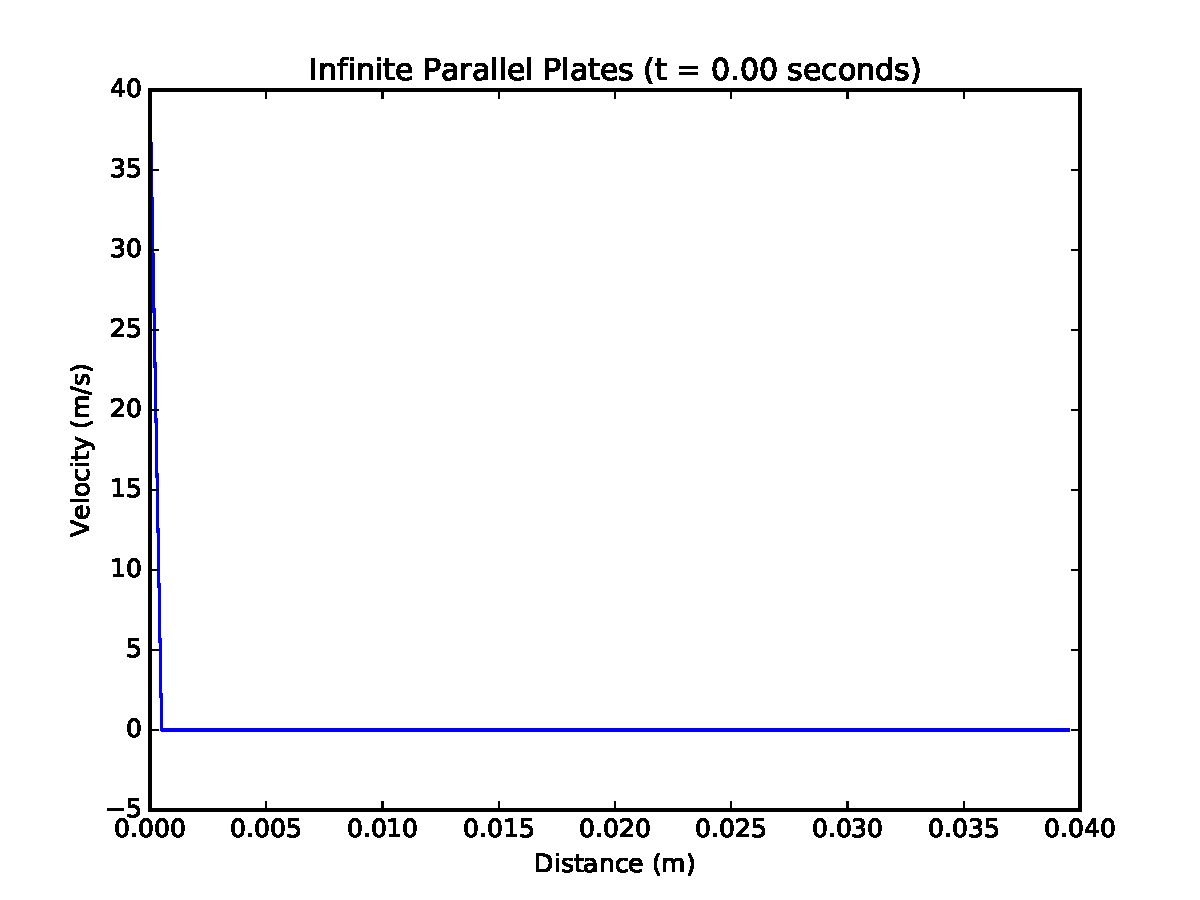
\includegraphics[width=.8\linewidth]{figs/0-00_sec_plot_FIT.pdf}
  \caption{$0.00$ seconds}
  \label{fig:0.0_forward}
\end{subfigure}%
\begin{subfigure}{.5\textwidth}
  \centering
  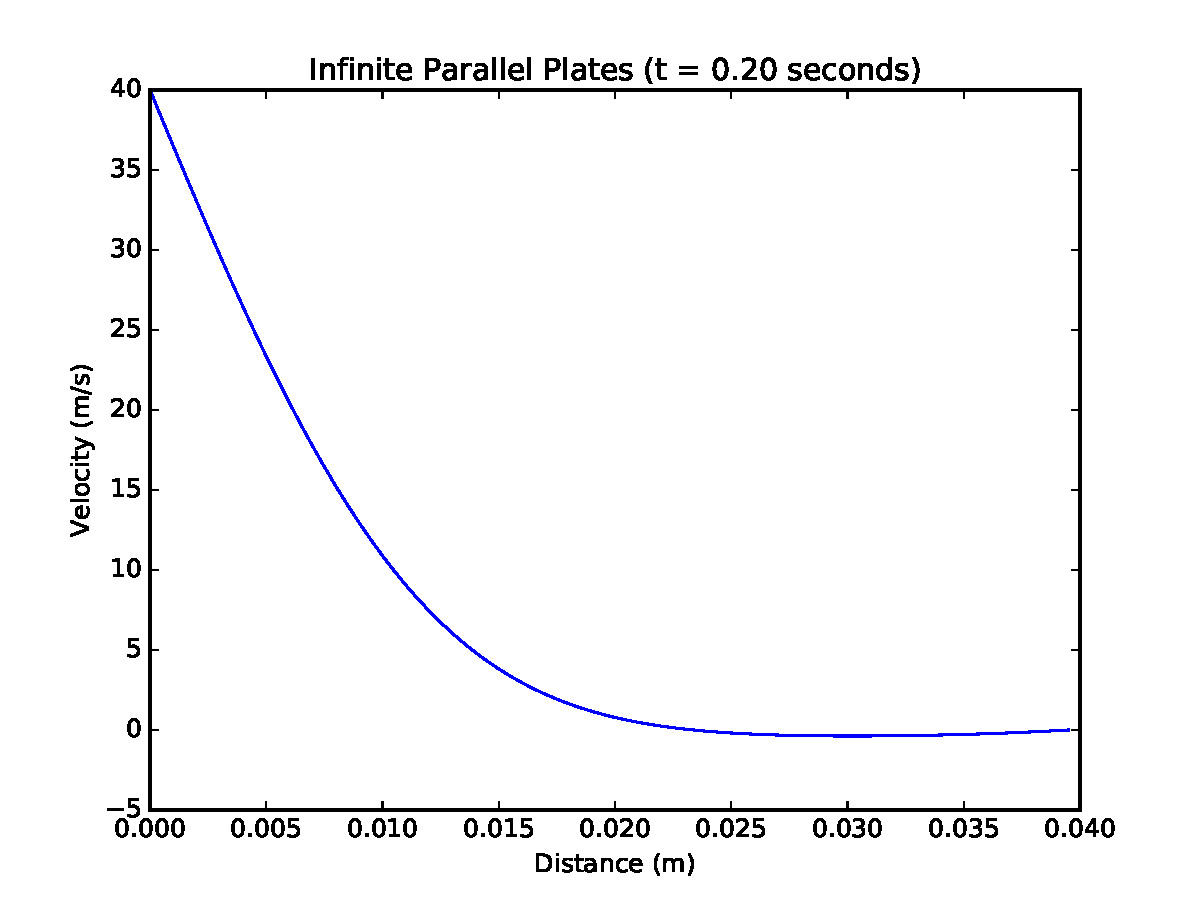
\includegraphics[width=.8\linewidth]{figs/0-20_sec_plot_FIT.pdf}
  \caption{$0.20$ seconds}
  \label{fig:0.2_forward}
\end{subfigure}
\begin{subfigure}{.5\textwidth}
  \centering
  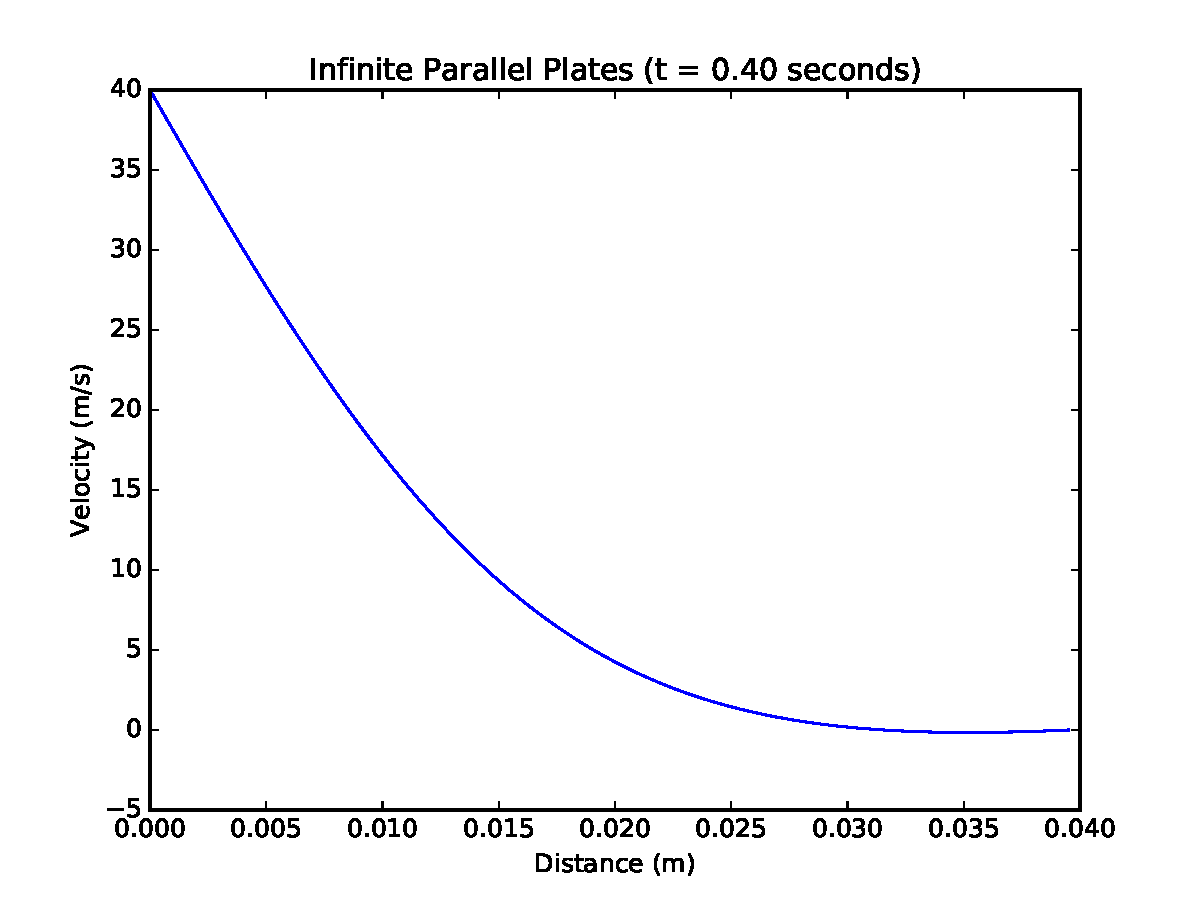
\includegraphics[width=.8\linewidth]{figs/0-40_sec_plot_FIT.pdf}
  \caption{$0.40$ seconds}
  \label{fig:0.4_forward}
\end{subfigure}
\begin{subfigure}{.5\textwidth}
  \centering
  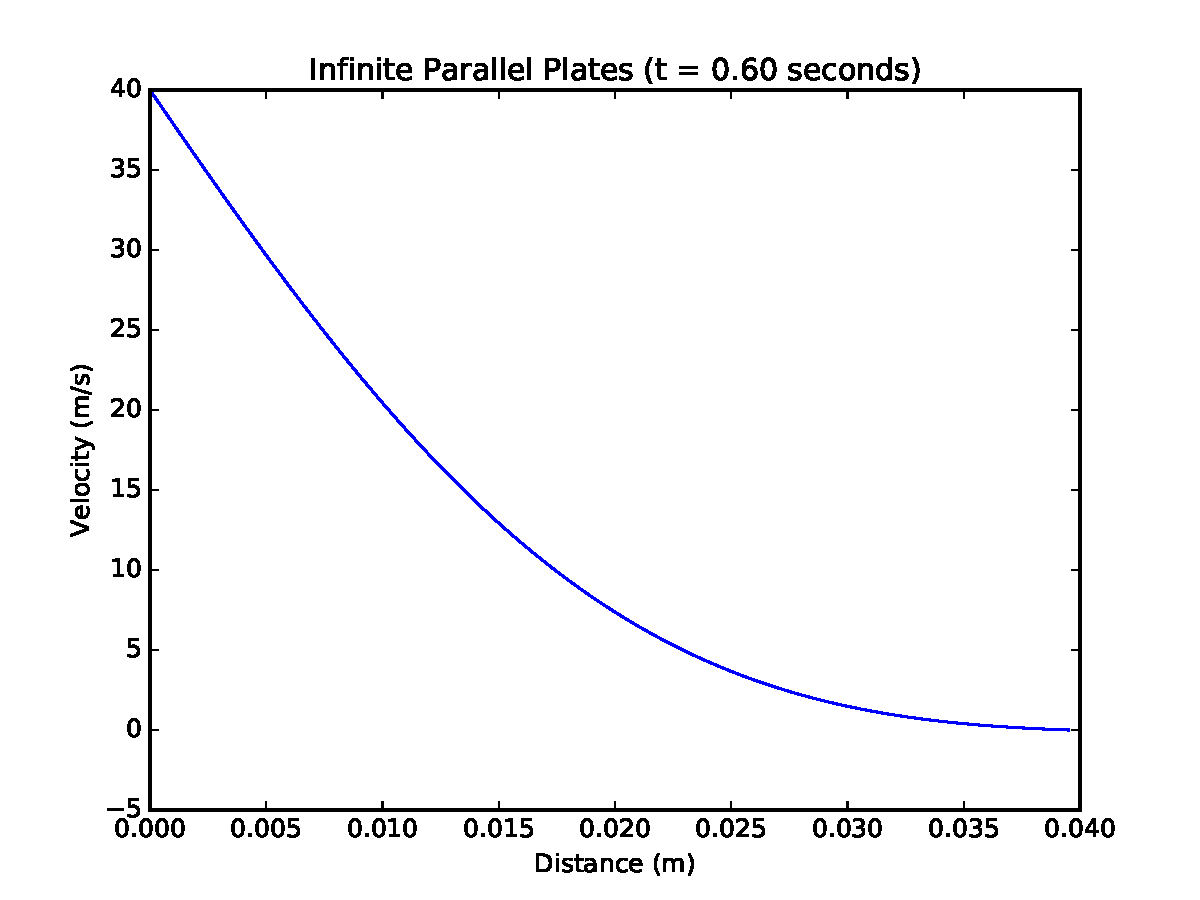
\includegraphics[width=.8\linewidth]{figs/0-60_sec_plot_FIT.pdf}
  \caption{$0.60$ seconds}
  \label{fig:0.6_forward}
\end{subfigure}
\begin{subfigure}{.5\textwidth}
  \centering
  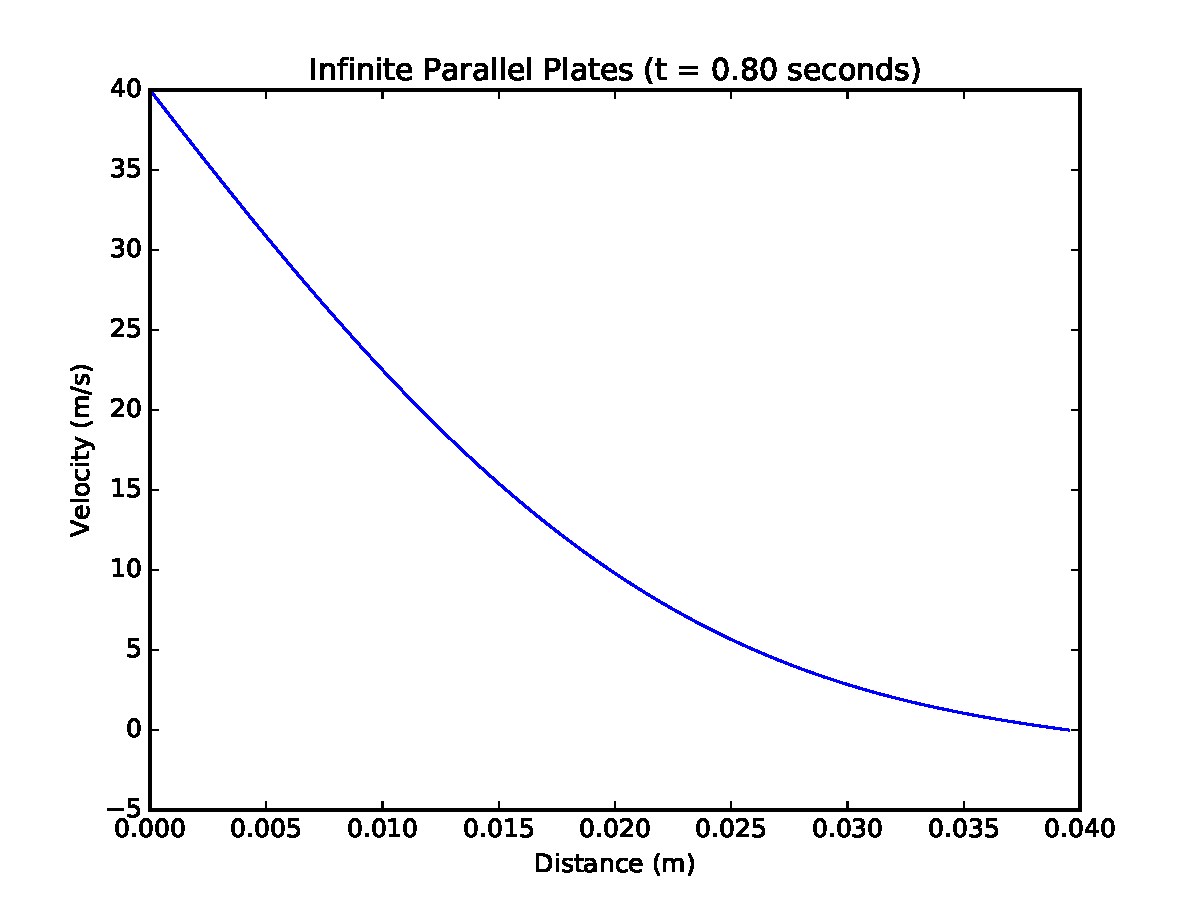
\includegraphics[width=.8\linewidth]{figs/0-80_sec_plot_FIT.pdf}
  \caption{$0.80$ seconds}
  \label{fig:0.8_forward}
\end{subfigure}
\begin{subfigure}{.5\textwidth}
  \centering
  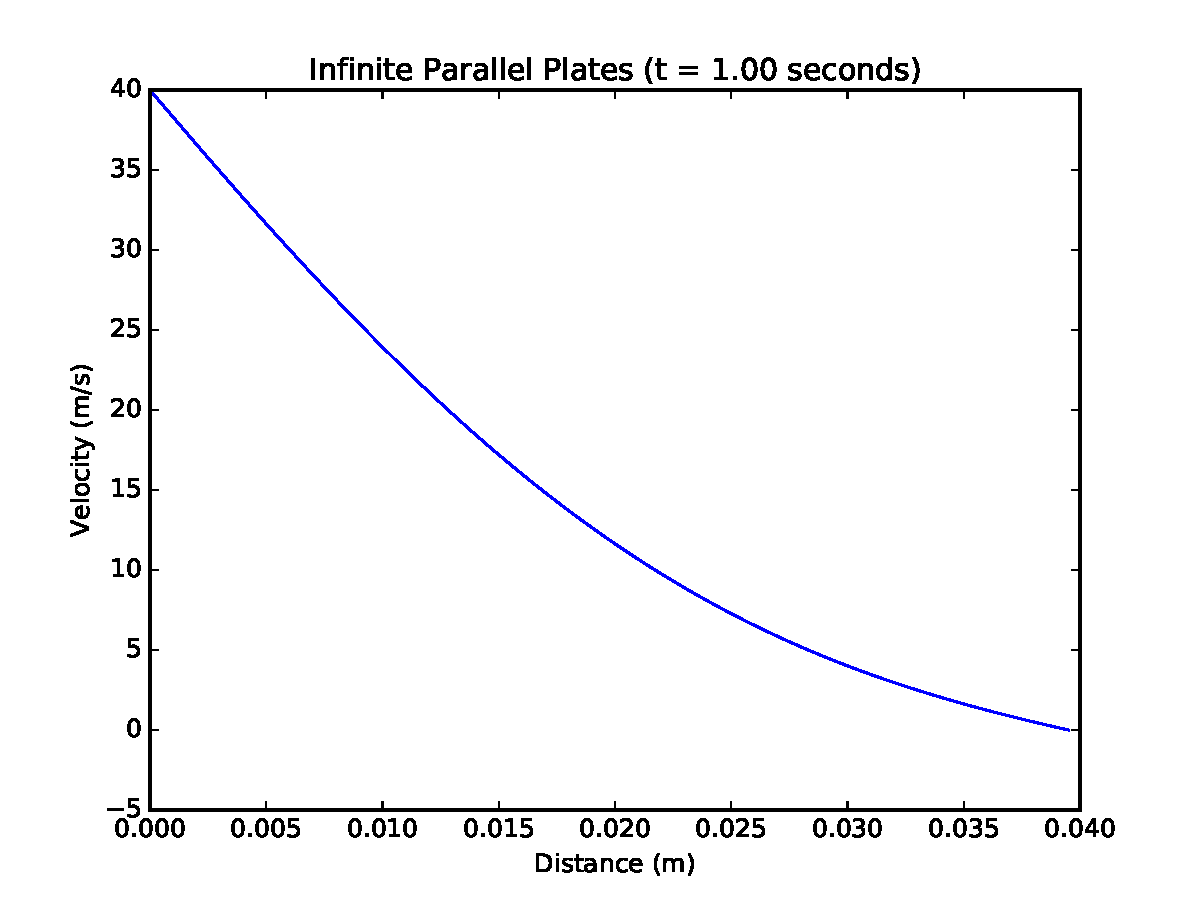
\includegraphics[width=.8\linewidth]{figs/1-00_sec_plot_FIT.pdf}
  \caption{$1.00$ seconds}
  \label{fig:1.0_forward}
\end{subfigure}
\caption{Forward in Time and Centered in Difference Infinite Parallel Plates Solution}
\label{fig:FIT}
\end{figure}
\end{solution}

\part Use the Crank-Nicolson implicit scheme to compute the velocity profiles and print them at the times specificed in part (b) for
\begin{itemize}
\item $\Delta t = 0.0005\ s$
\item $\Delta t = 0.00333\ s$
\end{itemize}
Compute and compare the CPU time for each method.

\begin{solution}
Before we can use the Crank-Nicolson method, we need to discretize Equation~(\ref{eq:plates}) using this scheme. To start off with, we get

\begin{align}
&\frac{u_{i,j}^{n+1}-u_{i,j}^{n}}{\Dt} = \underbrace{\frac{\nu}{2\Delta y^{2}}}_{\alpha}\left[u_{i,j+1}^{n}-2u_{i,j}^{n}+u_{i,j-1}^{n}+u_{i,j+1}^{n+1}-2u_{i,j}^{n+1}+u_{i,j-1}^{n+1} \right]
\intertext{which comes from the definition of the scheme. We can solve this by having all of the $u^{n+1}$ terms on one side and $u^{n}$ on the other. Doing so gives us}
&\underbrace{\left(\frac{1}{\Dt} + 2\alpha\right)}_{a}u_{i,j}^{n+1}\underbrace{-\alpha}_{d}u_{i,j+1}^{n+1} \underbrace{-\alpha}_{d}u_{i,j-1}^{n+1}= \underbrace{\left(\frac{1}{\Dt} - 2\alpha\right)u_{i,j}^{n}+\alpha u_{i,j+1}^{n}+\alpha u_{i,j-1}^{n}-\beta}_{b_{j}}
\end{align}
which is the discretized form of our original matrix. By looking at this, we can see that it looks {\em very similar} to the $\mathbf{A}\vec{x}=\vec{b}$ problem. In fact, we can exploit this so that we can solve it in that format. The terms in the underbrace are defined for the matrix below
\begin{align}
\mathbf{A} &= \left(\begin{matrix}a & d \\ d & a & d\\ & d & a & d\\ & & \ddots & \ddots & \ddots\\ & & & \ddots & \ddots & \ddots \\ & & & & d & a & d\\ & & & & & d & a\end{matrix}\right)
\intertext{where anything not in the tri-diagonal system is zero, where $a$ and $d$ were defined above. However, to constrain this system to work with the given boundary conditions, we need to make an adjustment to both $\mathbf{A}$ and $\vec{b}$, which are the following}
\mathbf{A} &= \left(\begin{matrix}1 &  \\  & a & d\\ & d & a & d\\ & & \ddots & \ddots & \ddots\\ & & & \ddots & \ddots & d \\ & & & & d & a & \\ & & & & &  & 1\end{matrix}\right)\\
\vec{b} &= \left(\begin{matrix}B.C.(1)\\ \left(\frac{1}{\Dt} - 2\alpha\right)u_{i,j}^{n}+\alpha u_{i,j+1}^{n}+\alpha u_{i,j-1}^{n}-\beta\\ \vdots\\ \vdots \\ b_{j}\\ \vdots \\ \vdots \\ \left(\frac{1}{\Dt} - 2\alpha\right)u_{i,j}^{n}+\alpha u_{i,j+1}^{n}+\alpha u_{i,j-1}^{n}-\beta\\ B.C.(2)\end{matrix} \right)
\end{align}
This keeps it so that $\mathbf{A}$ and $\vec{b}$ maintain the dimensions of the system which makes it easier in computations. $B.C.(1)$ and $B.C.(2)$ stand for the first and last boundary conditions, respectively, of the system, which occur at the ends. This allows us to create the linear system
\begin{align}
\mathbf{A}\vec{x} = \vec{b}
\end{align}
where the values in $\vec{x}$ are those values in the $u^{n+1}$ timestep. Therefore, in solving this system, we get the next values at each point in one step and it's not iterative as in the last problem. Using this technique, the solution to the above equation was achieved for each time step, which are discussed individually below.

{\em Note:} In these programs, the bottleneck of the system was in writing out the data. Therefore, to get a good ratio of the computational time of each, the same programs were run but without the File I/O. On top of this, each program was run a total of 10 times, and an average of the runtime was taken, which is the value that is reported below.

\begin{itemize}
\item $\Dt = 0.0005\ s$

The average runtime of this timestep was determined to be $0.0055291\ s$. This resulted in there being $2000$ time steps that were taken to get to the final solution. The results of this system are basically the same as the iteratve solution that was used in part $(b)$, and can be seen below.

\begin{figure}[H]
\begin{subfigure}{.5\textwidth}
  \centering
  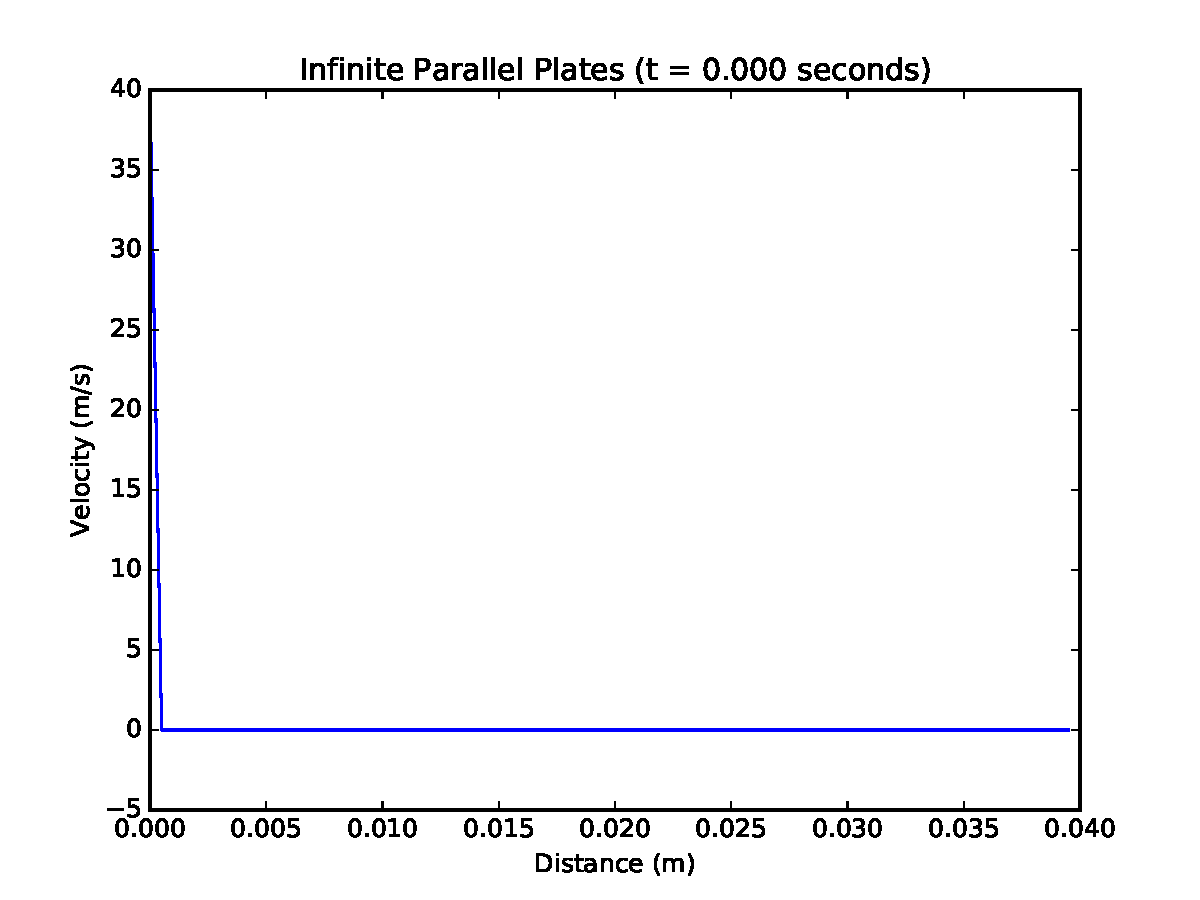
\includegraphics[width=.8\linewidth]{figs/0-000_sec_plot_CN1.pdf}
  \caption{$0.000$ seconds}
  \label{fig:0.0_CN1}
\end{subfigure}%
\begin{subfigure}{.5\textwidth}
  \centering
  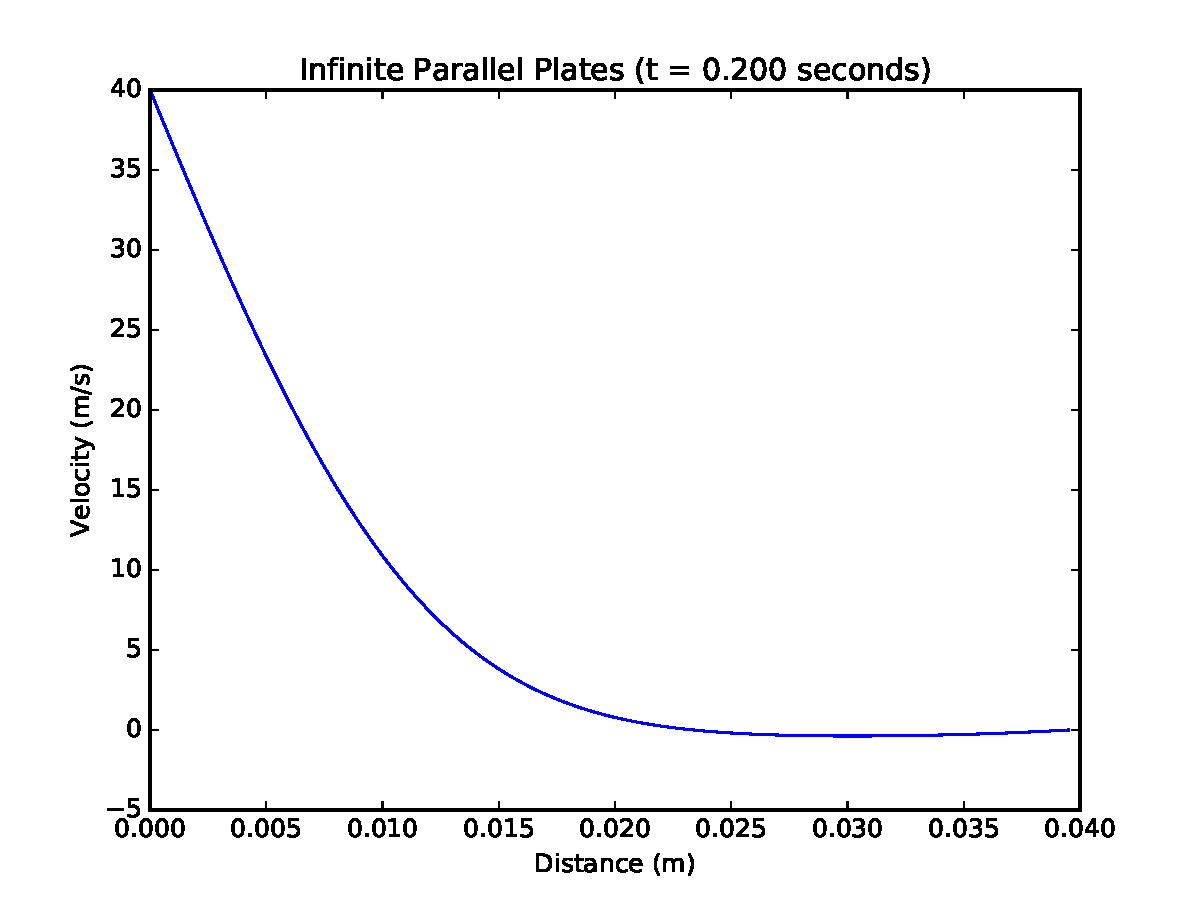
\includegraphics[width=.8\linewidth]{figs/0-200_sec_plot_CN1.pdf}
  \caption{$0.200$ seconds}
  \label{fig:0.2_CN1}
\end{subfigure}
\begin{subfigure}{.5\textwidth}
  \centering
  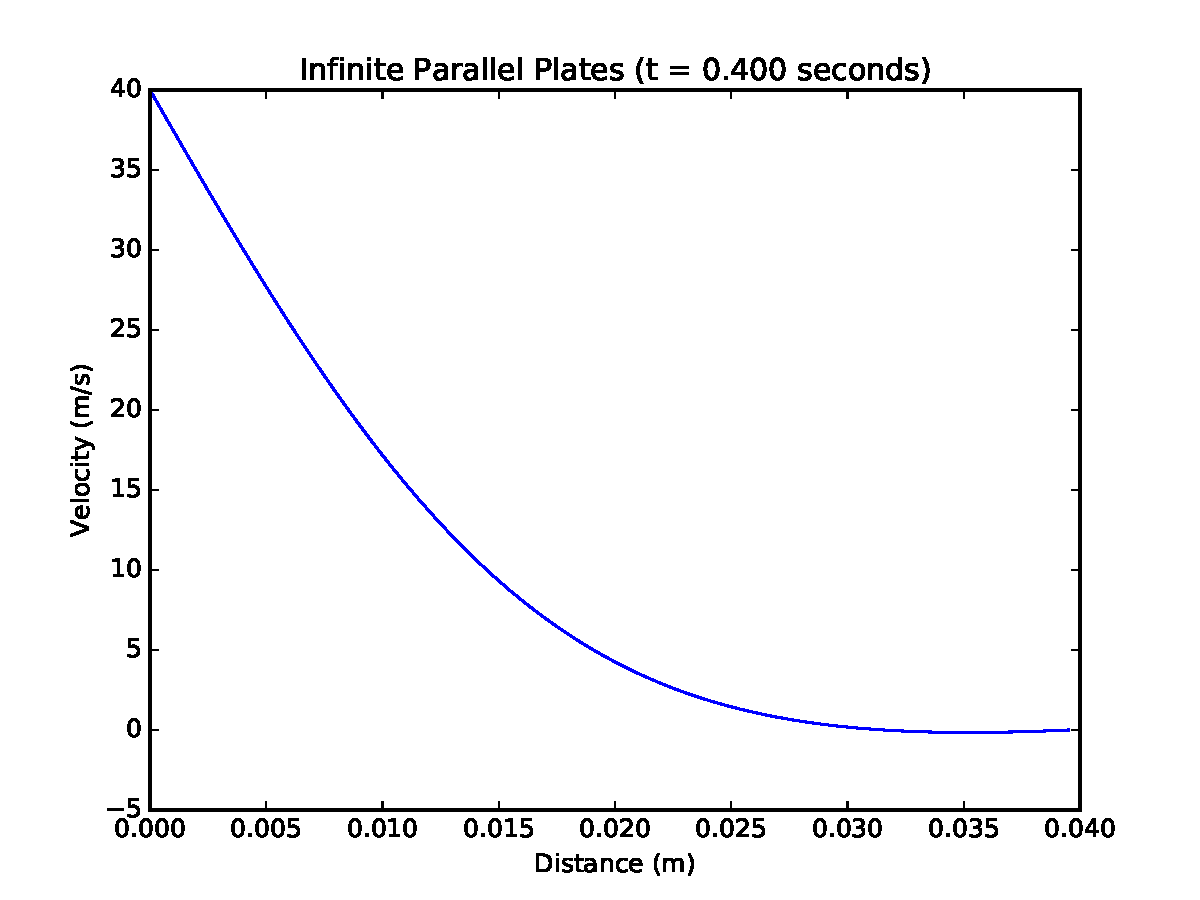
\includegraphics[width=.8\linewidth]{figs/0-400_sec_plot_CN1.pdf}
  \caption{$0.400$ seconds}
  \label{fig:0.4_CN1}
\end{subfigure}
\begin{subfigure}{.5\textwidth}
  \centering
  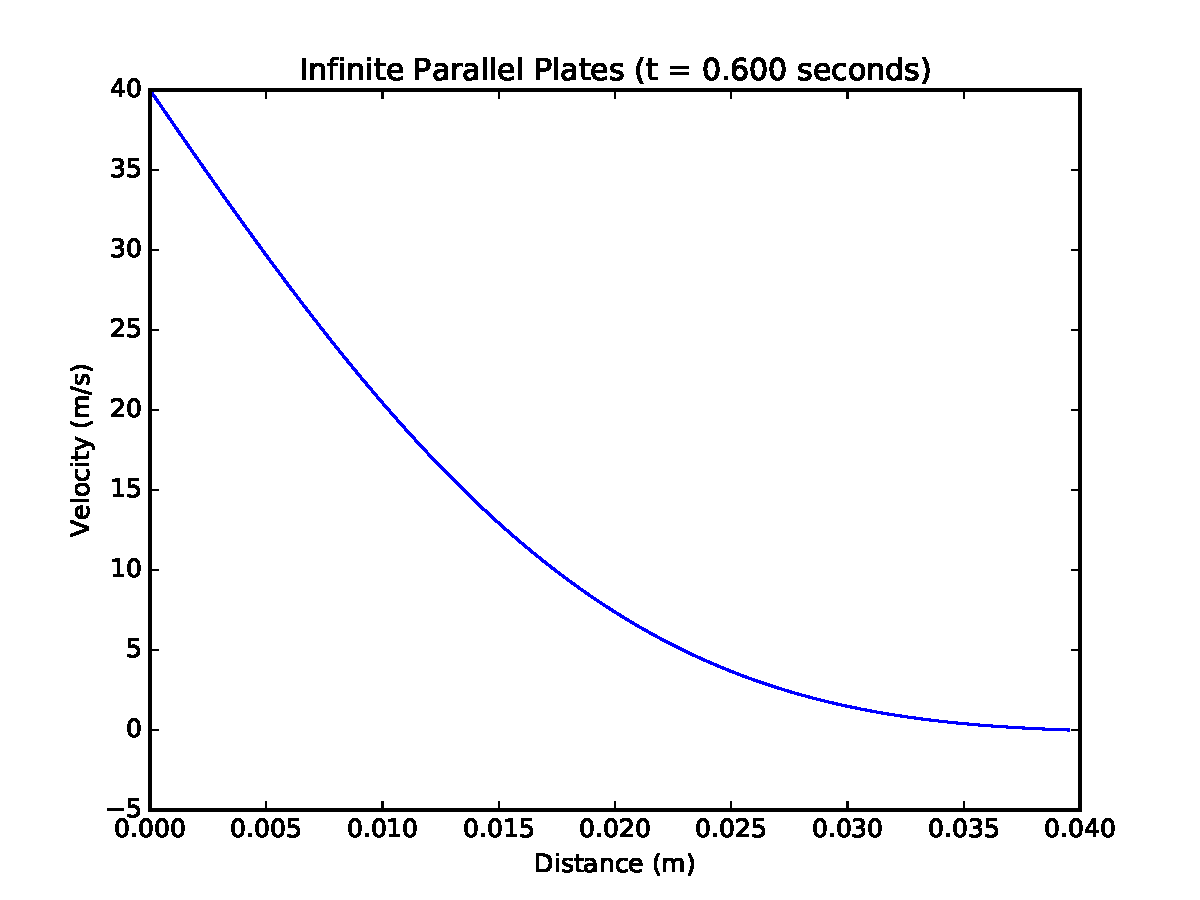
\includegraphics[width=.8\linewidth]{figs/0-600_sec_plot_CN1.pdf}
  \caption{$0.600$ seconds}
  \label{fig:0.6_CN1}
\end{subfigure}
\begin{subfigure}{.5\textwidth}
  \centering
  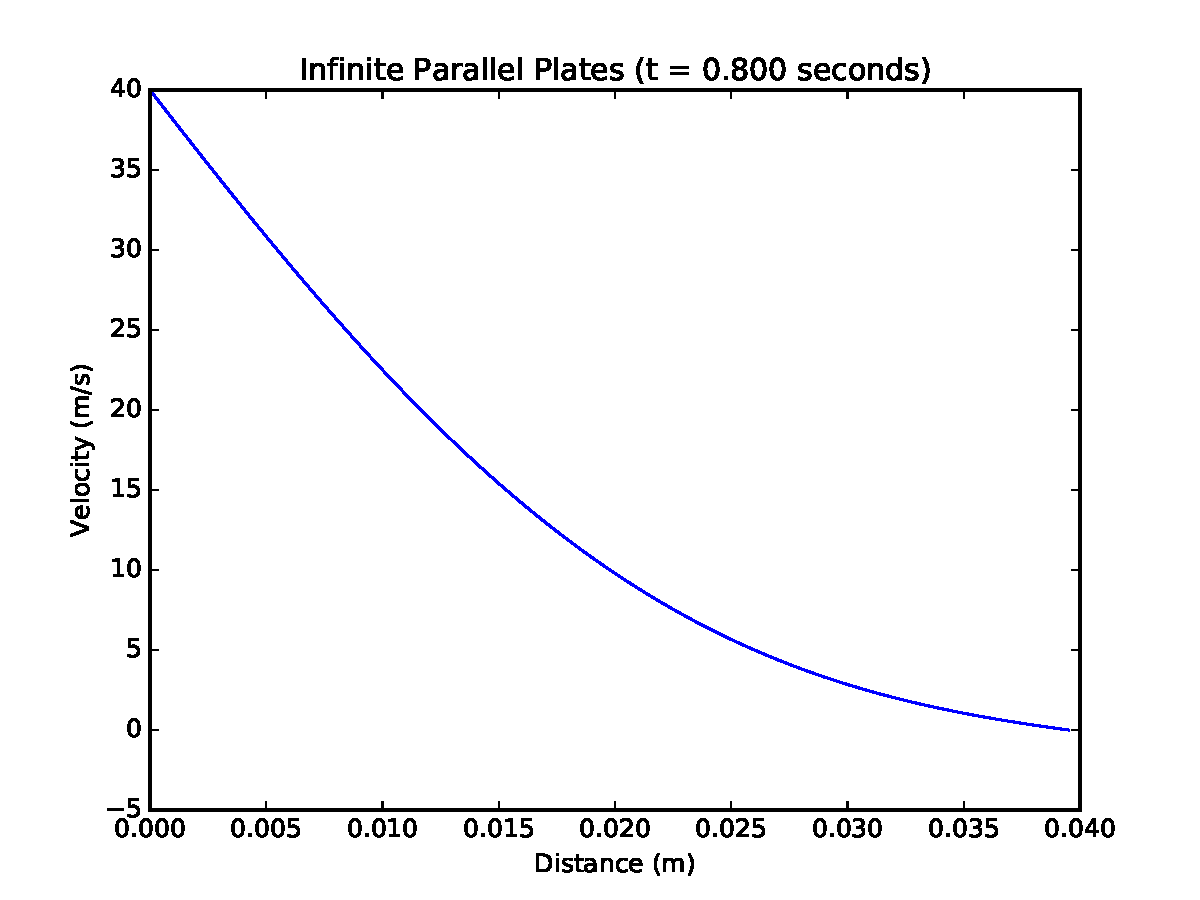
\includegraphics[width=.8\linewidth]{figs/0-800_sec_plot_CN1.pdf}
  \caption{$0.800$ seconds}
  \label{fig:0.8_CN1}
\end{subfigure}
\begin{subfigure}{.5\textwidth}
  \centering
  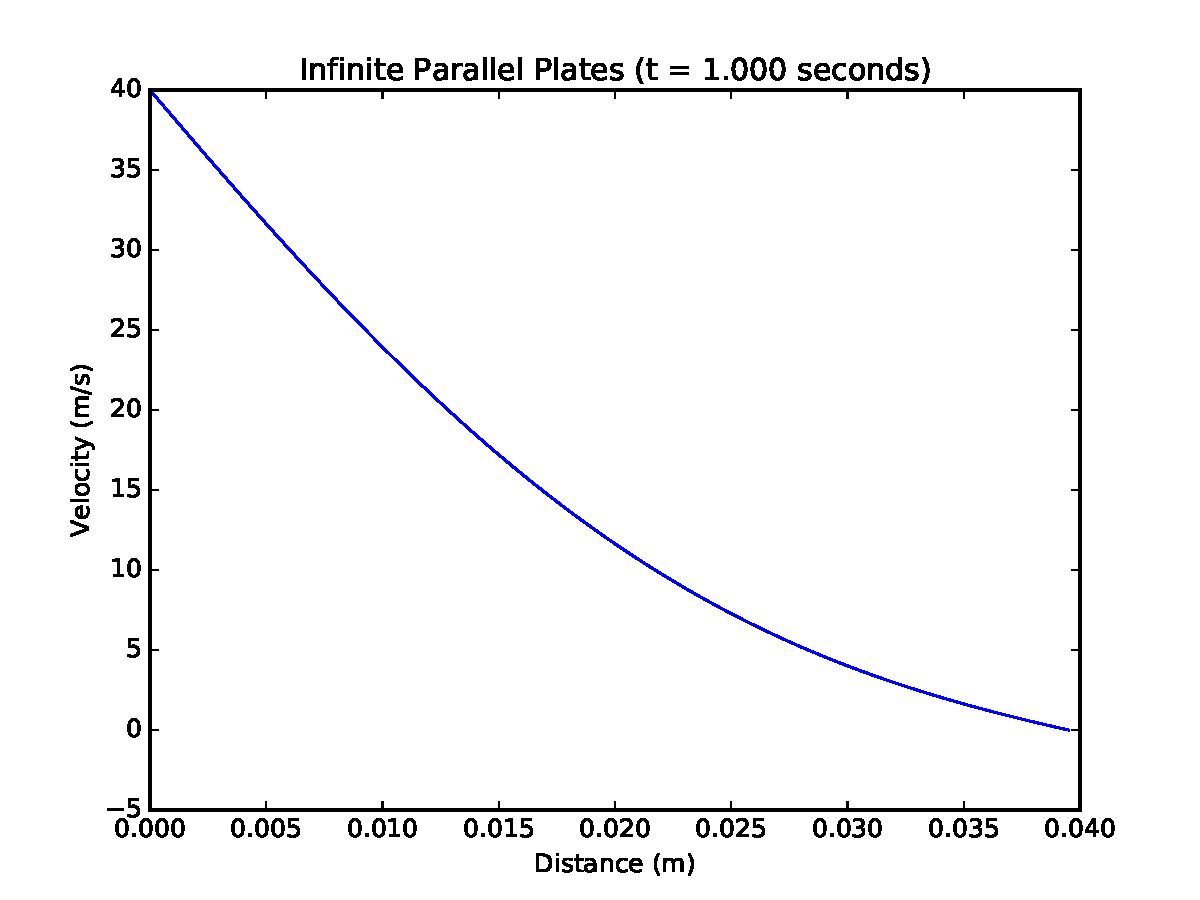
\includegraphics[width=.8\linewidth]{figs/1-000_sec_plot_CN1.pdf}
  \caption{$1.000$ seconds}
  \label{fig:1.0_CN1}
\end{subfigure}
\caption{Crank-Nicolson $\Dt = 0.0005\ s$ Infinite Parallel Plates Solution}
\label{fig:CN1}
\end{figure}

\item $\Dt = 0.00333\ s$

The average runtime of this timestep was determined to be $0.0008473\ s$. This resulted in there being only $300$ time steps to the final solution. This is approximately 15\% the number of timesteps as required in the above example. If we take the runtime of $\Dt = 0.0005\ s$ and multiply it by 15\%, since this one should be approximately 15\% of the above runtime, we get a value that is almost exactly ours ($0.0008295\ s$). 

The results of this timestep were almost exactly the same as the above two solutions. One thing to note is that even though this asked for them in the same times, it was impossible to achieve this as no combination of $\Dt$ would give those values when starting from 0. Therefore, the time values that are closest were reported and can be seen below.

\begin{figure}[H]
\begin{subfigure}{.5\textwidth}
  \centering
  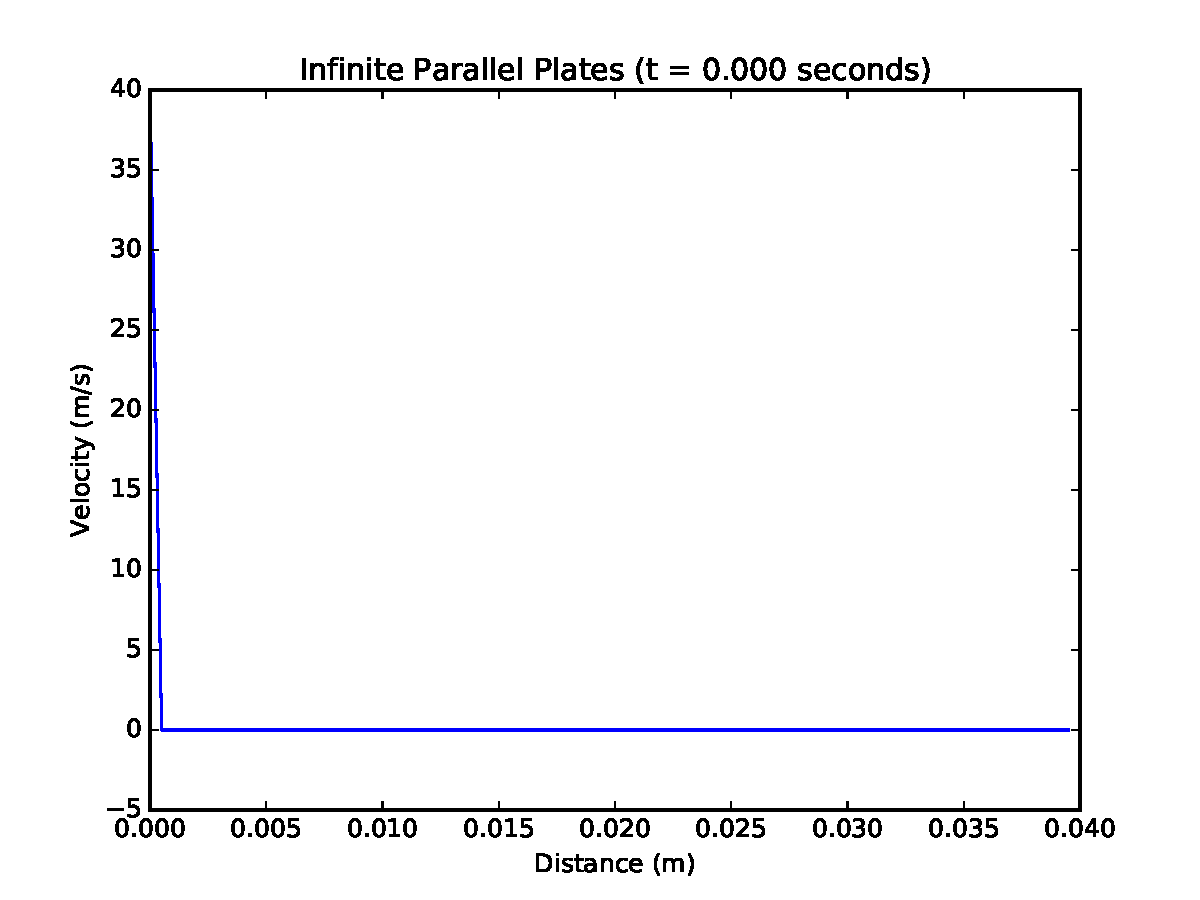
\includegraphics[width=.8\linewidth]{figs/0-000_sec_plot_CN2.pdf}
  \caption{$0.000$ seconds}
  \label{fig:0.0_CN2}
\end{subfigure}%
\begin{subfigure}{.5\textwidth}
  \centering
  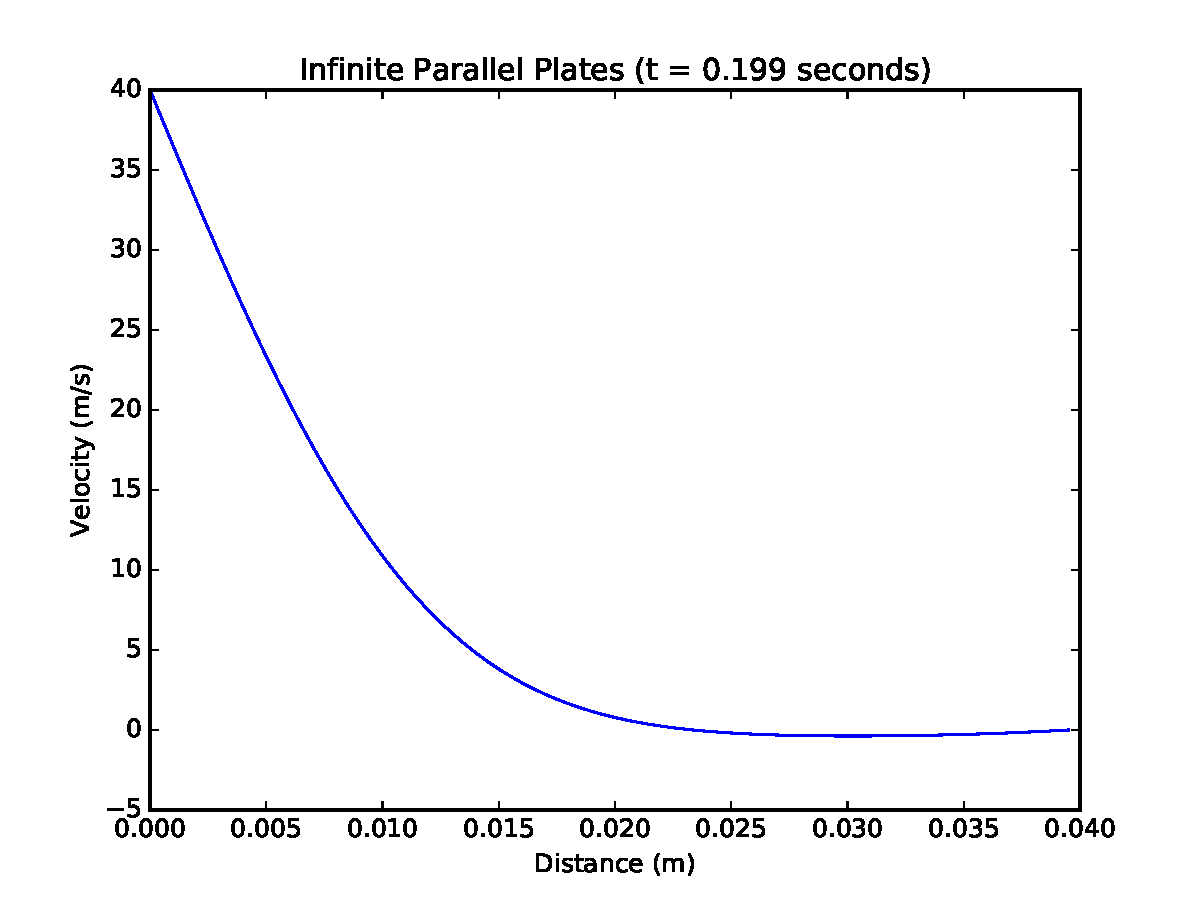
\includegraphics[width=.8\linewidth]{figs/0-199_sec_plot_CN2.pdf}
  \caption{$0.199$ seconds}
  \label{fig:0.2_CN2}
\end{subfigure}
\begin{subfigure}{.5\textwidth}
  \centering
  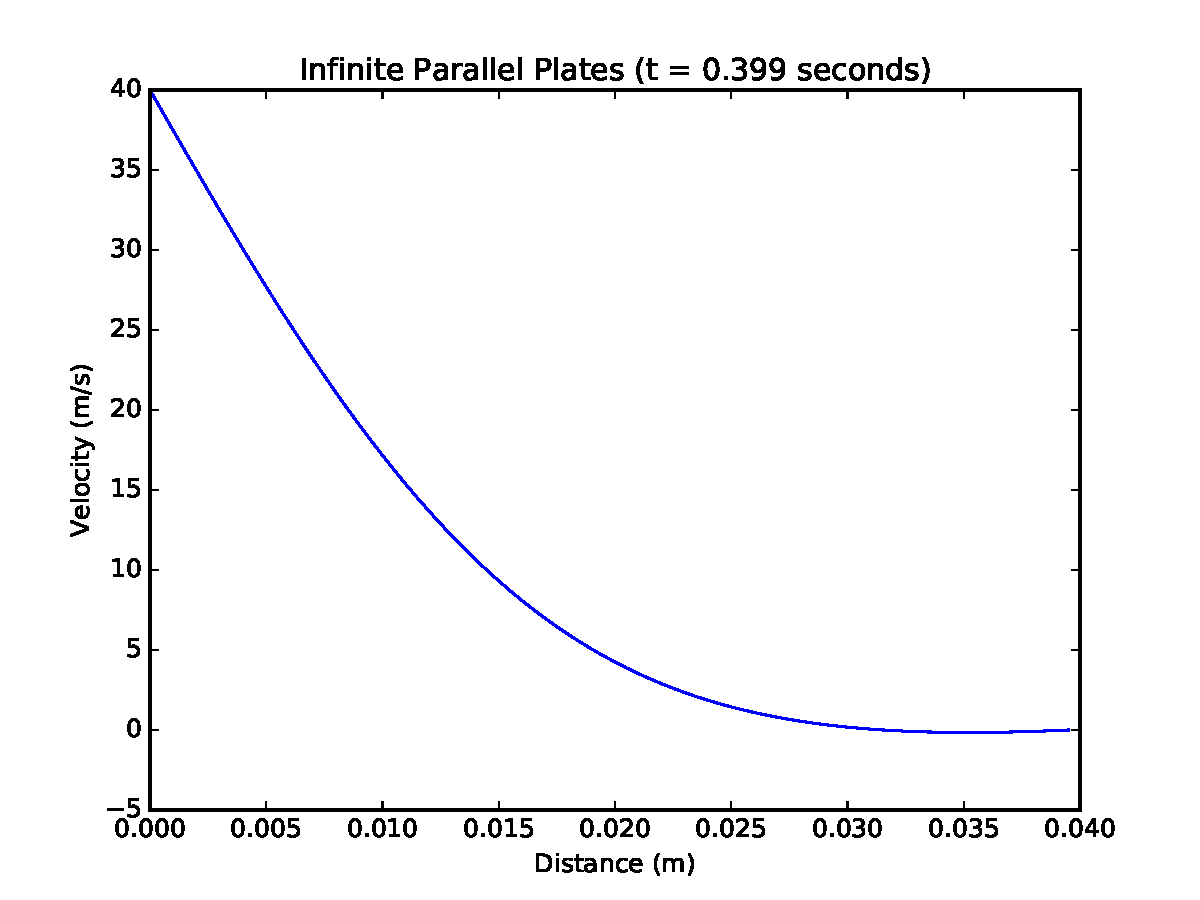
\includegraphics[width=.8\linewidth]{figs/0-399_sec_plot_CN2.pdf}
  \caption{$0.399$ seconds}
  \label{fig:0.4_CN2}
\end{subfigure}
\begin{subfigure}{.5\textwidth}
  \centering
  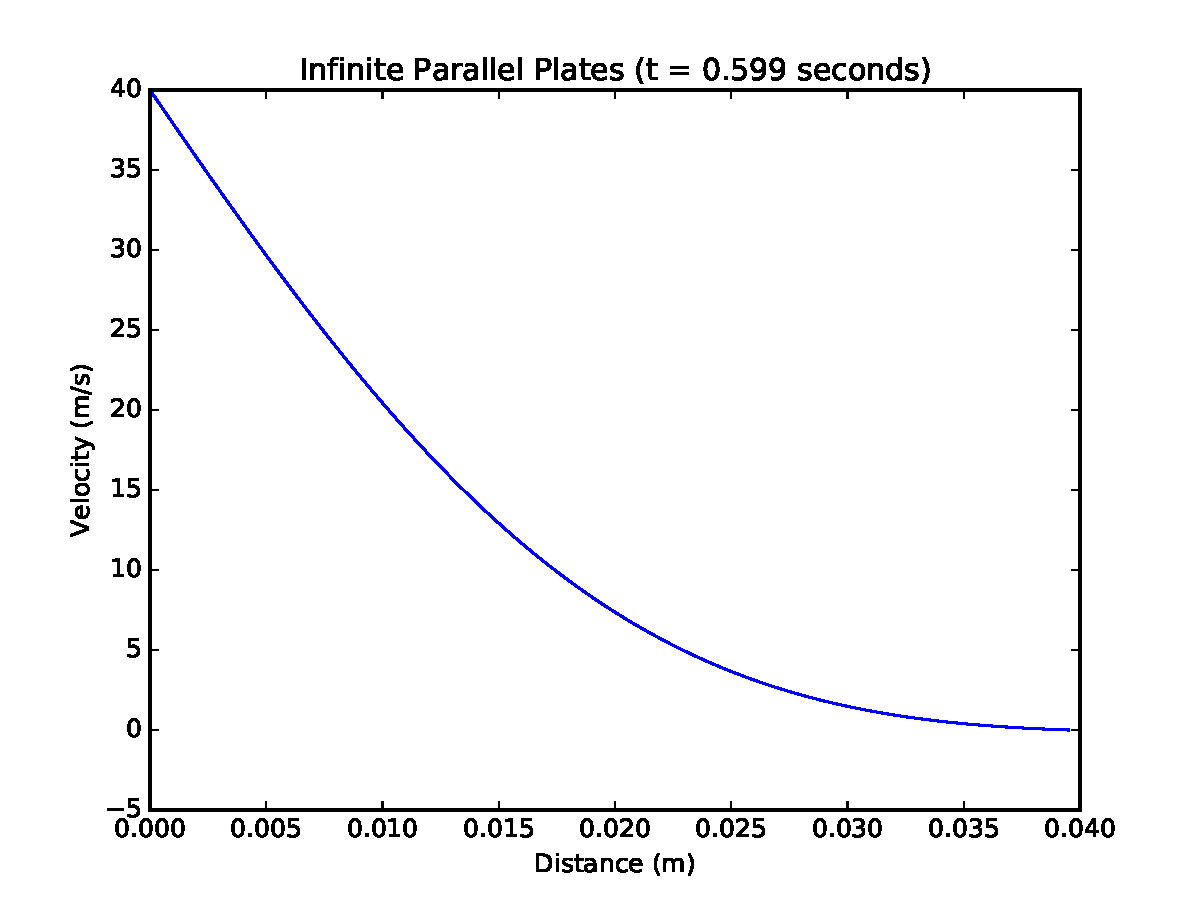
\includegraphics[width=.8\linewidth]{figs/0-599_sec_plot_CN2.pdf}
  \caption{$0.599$ seconds}
  \label{fig:0.6_CN2}
\end{subfigure}
\begin{subfigure}{.5\textwidth}
  \centering
  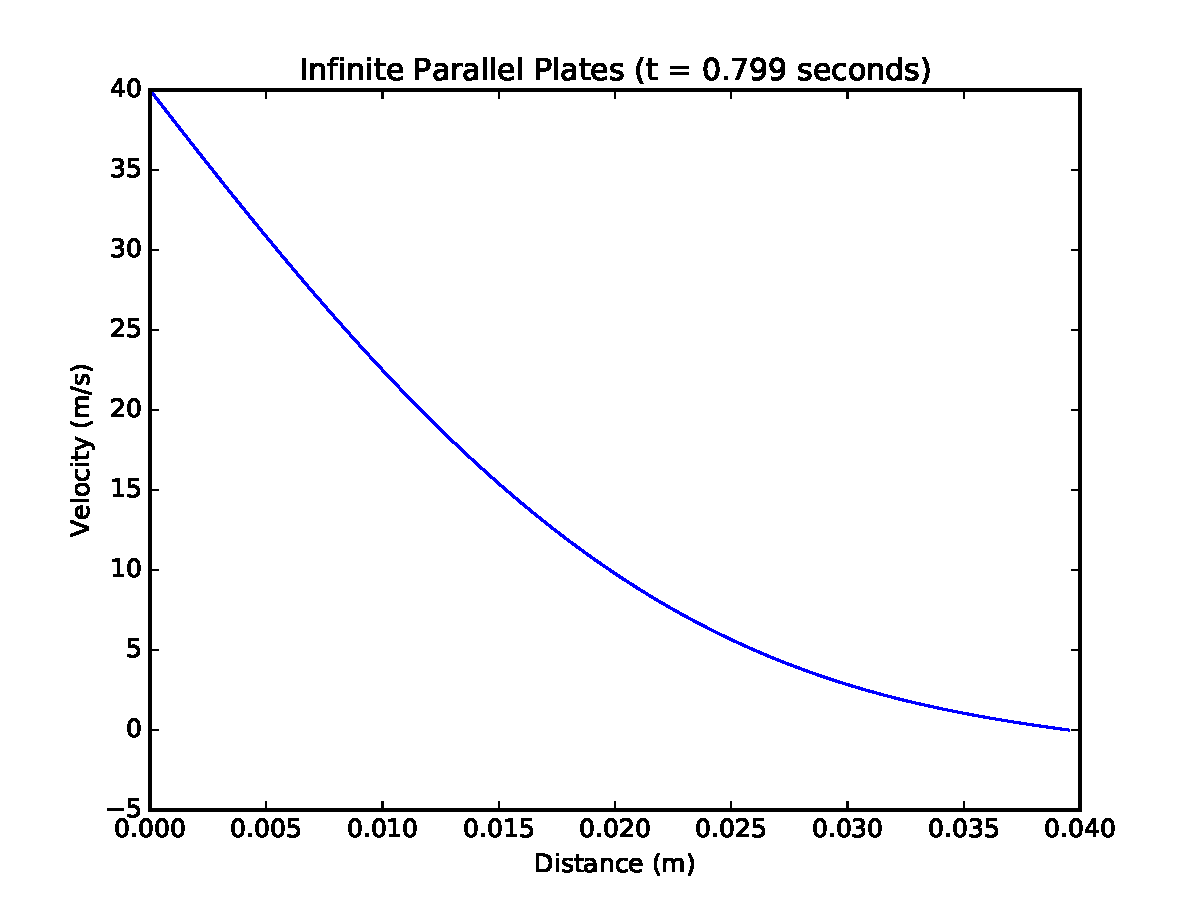
\includegraphics[width=.8\linewidth]{figs/0-799_sec_plot_CN2.pdf}
  \caption{$0.799$ seconds}
  \label{fig:0.8_CN2}
\end{subfigure}
\begin{subfigure}{.5\textwidth}
  \centering
  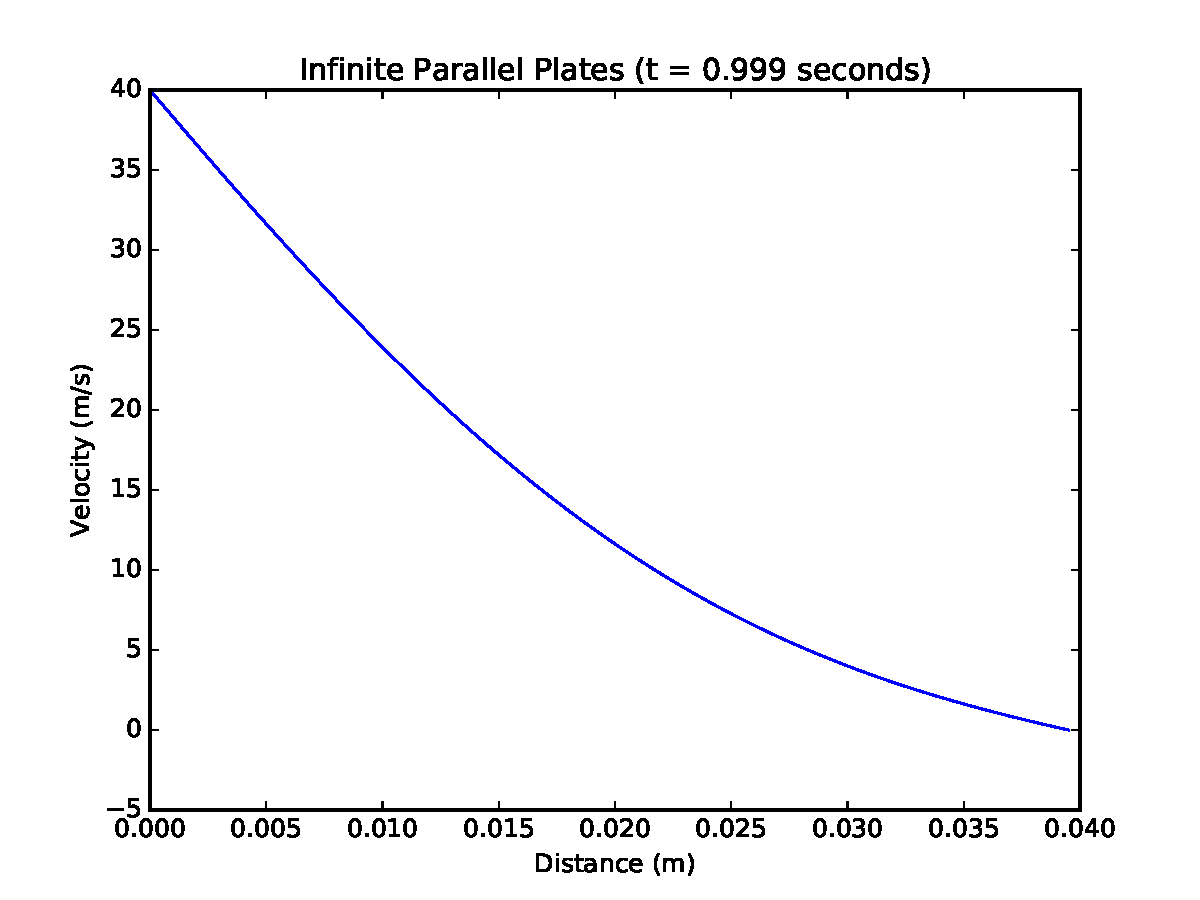
\includegraphics[width=.8\linewidth]{figs/0-999_sec_plot_CN2.pdf}
  \caption{$0.999$ seconds}
  \label{fig:1.0_CN2}
\end{subfigure}
\caption{Crank-Nicolson $\Dt = 0.00333\ s$ Infinite Parallel Plates Solution}
\label{fig:CN2}
\end{figure}
\end{itemize}
\end{solution}

\end{parts}
\ \newpage
\titledquestion{Heated Bar}
A long, rectangular bar has dimensions of $L_{x}$ by $L_{y}$, as shown in Figure~\ref{fig:bar}. The bar is initially heated to a temperature $T_{0}$. Subsequently, its surfaces are subjected to the constant temperature of $T_{1},\ T_{2},\ T_{3},$ and $T_{4}$ as depicted in the figure.

\begin{figure}[H]
\centering
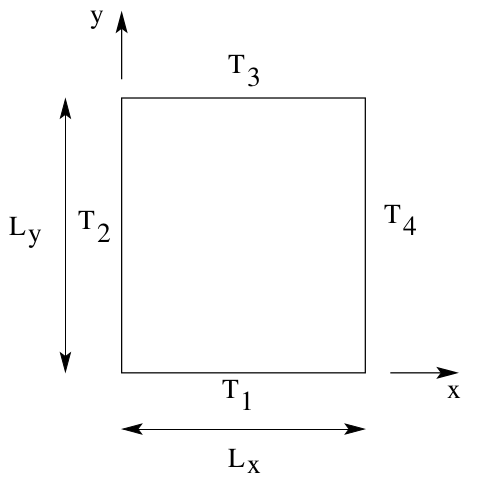
\includegraphics[width=.4\textwidth]{fig1.png}
\caption{Bar Dimensions}
\label{fig:bar}
\end{figure}

The problem is governed by the 2D unsteady heat equation given by

\begin{align}
\frac{\partial T}{\partial t} &= \alpha\left(\frac{\partial ^{2}T}{\partial x^{2}} + \frac{\partial^{2}T}{\partial y^{2}}\right)\label{eq:heateq}
\end{align}

The bar is composed of copper with constant thermal conductivity of $380\ \unitfrac{W}{m^{\circ}C}$ and a constant thermal diffusivity of $1.1234\times 10^{-4}\ \unitfrac{m^{2}}{s}$. The bar has dimensions of $L_{x}=0.3\ \text{m}$ and $L_{y} = 0.4\ \text{m}$.

Use the ADI (Alternating Direction Implicit) scheme with timesteps of $0.1\ s$ and $0.5\ s$ and a computational grid with $N_{x}=61$ and $N_{y}=81$ grid points to compute the transient solution. The initial condition and boundary conditions are given by: $T_{0}= 0.0\ ^{\circ}\text{C},\ T_{1}=40.0\ ^{\circ}\text{C},\ T_{2}=0.0\ ^{\circ}\text{C},\ T_{3}=10.0\ ^{\circ}\text{C},$ and $T_{4}=0.0\ ^{\circ}\text{C}$.

Print contour plots (of isotemperature lines) corresponding to $t=0.5\ s, t=10.0\ s, t=20.0\ s, t=40.0\ s$ and steady state. Assume the simulation has reached steady state when the total variation (TV) in the temperature from one time step to the next is less than $0.0001\ ^{\circ}\text{C}$, where

\begin{align}
\text{TV} &= \frac{1}{N_{x}N_{y}}\sum_{j=2}^{N_{y}}\sum_{i=2}^{N_{x}}\left| T_{i,j}^{n+1}-T_{i,j}^{n}\right|\label{eq:steady_state}
\end{align}

Discuss your results

\begin{solution}
In Equation~(\ref{eq:heateq}), $\alpha$ is the diffusivity of the material. It will be left as $\alpha$ throughout the mathematics of this section, though is defined numerically in the code as $1.1234\times 10^{-4}\ \unitfrac{m^{2}}{s}$, which above was stated as being for copper.

The ADI scheme is defined in the following way

\begin{align}
\frac{u_{i,j}^{n+\frac{1}{2}}-u_{i,j}^{n}}{\Dtp} &= \left( \delta_{x}^{2}u_{i,j}^{n+\frac{1}{2}}+\delta_{y}^{2}u_{i,j}^{n}\right)\\
\frac{u_{i,j}^{n+1}-u_{i,j}^{n+\frac{1}{2}}}{\Dtp} &= \left( \delta_{x}^{2}u_{i,j}^{n+\frac{1}{2}}+\delta_{y}^{2}u_{i,j}^{n+1}\right)
\intertext{where $\delta_{p}$ is the central difference operator in the $p$ dimeinson, and $\Dtp$ is $\Dt /2$. In expanding these for Equation~(\ref{eq:heateq}), we get}
\frac{u_{i,j}^{n+\frac{1}{2}}-u_{i,j}^{n}}{\Dtp} &= \alpha\left(\frac{u_{i+1,j}^{n+\frac{1}{2}}-2u_{i,j}^{n+\frac{1}{2}}+u_{i-1,j}^{n+\frac{1}{2}}}{\Dx^{2}} + \frac{u_{i,j+1}^{n}-2u_{i,j}^{n}+u_{i,j-1}^{n}}{\Dy^{2}}\right)\label{eq:adix}\\
\frac{u_{i,j}^{n+1}-u_{i,j}^{n+\frac{1}{2}}}{\Dtp} &= \alpha\left(\frac{u_{i+1,j}^{n+\frac{1}{2}}-2u_{i,j}^{n+\frac{1}{2}}+u_{i-1,j}^{n+\frac{1}{2}}}{\Dx^{2}} + \frac{u_{i,j+1}^{n+1}-2u_{i,j}^{n+1}+u_{i,j-1}^{n+1}}{\Dy^{2}}\right)\label{eq:adiy}
\end{align}
In solving Equation~(\ref{eq:adix}) for the $u^{n+\frac{1}{2}}$ terms on the left and the $u^{n}$ terms on the right, we get
\begin{align}
\underbrace{\left(\frac{1}{\Dtp} + \frac{2\alpha}{\Dx^{2}}\right)}_{a_{x}}u_{i,j}^{n+\frac{1}{2}} \underbrace{-\frac{\alpha}{\Dx^{2}}}_{d_{x}}u_{i+1,j}^{n+\frac{1}{2}}\underbrace{-\frac{\alpha}{\Dx^{2}}}_{d_{x}}u_{i-1,j}^{n+\frac{1}{2}} &= \underbrace{\left(\frac{1}{\Dtp}-\frac{2\alpha}{\Dy^{2}}\right)u_{i,j}^{n} + \frac{\alpha}{\Dy^{2}}u_{i,j+1}^{n} + \frac{\alpha}{\Dy^{2}}u_{i,j-1}^{n}}_{\vec{b}}\label{eq:adix_s}
\intertext{likewise, for Equation~(\ref{eq:adiy})}
\underbrace{\left(\frac{1}{\Dtp} + \frac{2\alpha}{\Dy^{2}}\right)}_{a_{y}}u_{i,j}^{n+1} \underbrace{-\frac{\alpha}{\Dy^{2}}}_{d_{y}}u_{i,j+1}^{n+1}\underbrace{-\frac{\alpha}{\Dy^{2}}}_{d_{y}}u_{i,j-1}^{n+1} &= \underbrace{\left(\frac{1}{\Dtp}-\frac{2\alpha}{\Dx^{2}}\right)u_{i,j}^{n+\frac{1}{2}} + \frac{\alpha}{\Dx^{2}}u_{i+1,j}^{n+\frac{1}{2}} + \frac{\alpha}{\Dx^{2}}u_{i-1,j}^{n+\frac{1}{2}}}_{\vec{b}}\label{eq:adiy_s}
\end{align}
With this, we can build the two tri-diagonal systems
\begin{align}
\mathbf{A}_{x}\vec{x} &= \vec{b}\label{eq:axb_x}\\
\mathbf{A}_{y}\vec{x} &= \vec{b}\label{eq:axb_y}
\end{align}
where we will have to first solve Equation~(\ref{eq:axb_x}) and then use that solution to build $\vec{b}$ in Equation~(\ref{eq:axb_y}). {\em Note}: Just like in the previous problem, we have to constrain $\mathbf{A}_{x}$, $\mathbf{A}_{y}$, and $\vec{b}$ to the boundary conditions. This is done by setting $d_{x}$ and $d_{y}$ to be zero at the correspoinding points, $a_{x}$ and $a_{y}$ to being 1, and $b_{j}$ to the value of the boundary condition.

The question asks to run the simulation for $\Dt = 0.1\ s$ and $\Dt = 0.5\ s$, and it was unstable for $\Dt = 0.5\ s$ past the $10.0\ s$ mark. The results below are for the stable iterations of $\Dt = 0.1\ s$ since the results were not readable or even interpretable for the other case.

Figure~\ref{fig:0.50} shows the time for $0.500\ s$. At this point in the simulation, there is not a lot that has changed in the overall problem. The inner portion of the bar is beginning to heat up as the heat propogates from the $T_{1}$ and $T_{3}$ edges. 

For Figure~\ref{fig:10.0}, $t = 10.0\ s$ and the bar has heated up enough to where it has almost removed any initial conditions that were on the bar. It is completely gone at $t = 20.0\ s$ and the heated boundaries are continually heating up more of the plate, as Figure~\ref{fig:20.0} shows. 

By the time the system gets to $t = 40.0\ s$ in Figure~\ref{fig:40.0}, it starts to slow down in how much the system is changing, but it still hasn't reached the ``steady state'' yet, as defined with Equation~(\ref{eq:steady_state}). From this point, the system was continually solved until the steady state was achieved, which was at $t = 179.6\ s$. While Figure~\ref{fig:steady_state} looks a lot different than $t = 40.0\ s$, it took a long time to get to its steady state, so there was not {\em that much} change between the two.


\begin{figure}[H]
\centering
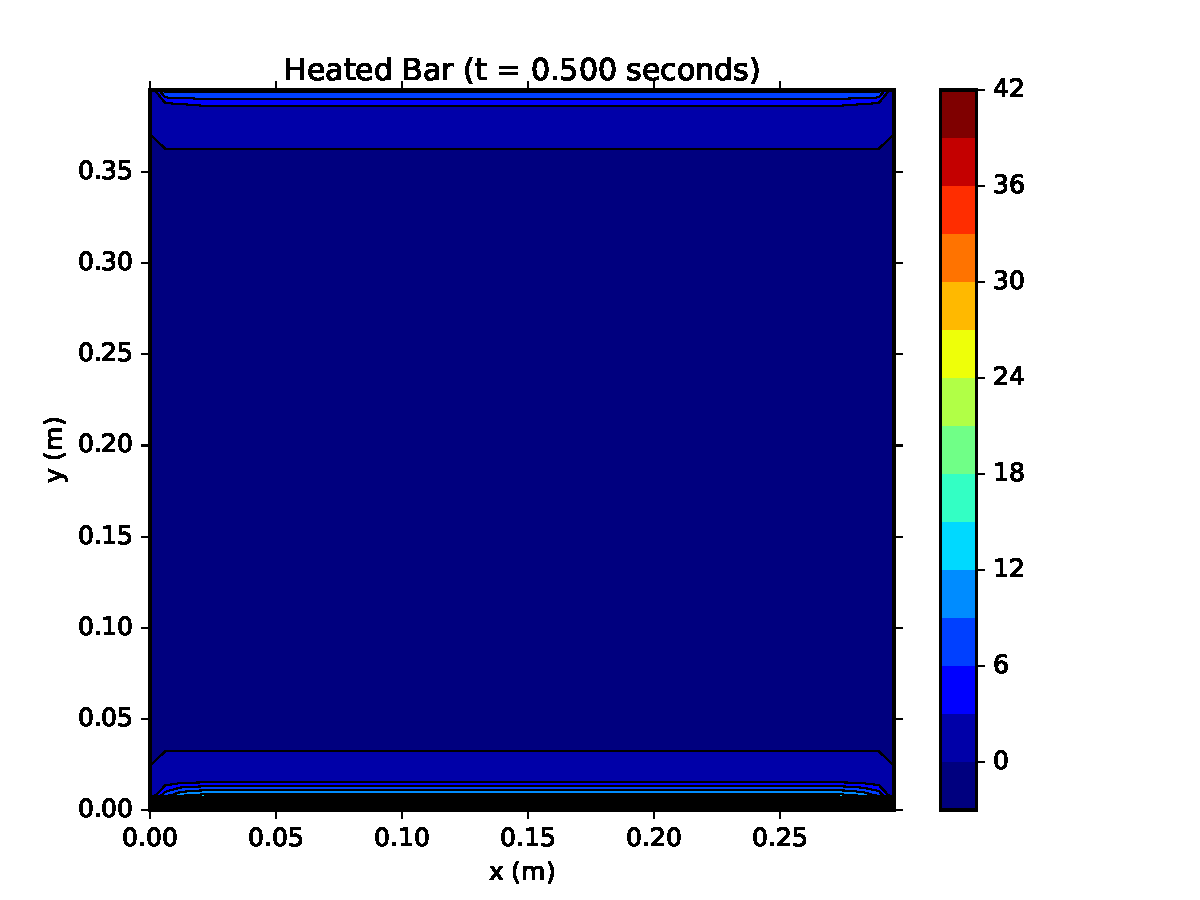
\includegraphics[width=.8\linewidth]{figs/0-500_sec_heat-eq_colorplot.pdf}
\caption{Heated Bar $t=0.500\ s$}
\label{fig:0.50}
\end{figure}


\begin{figure}[H]
\centering
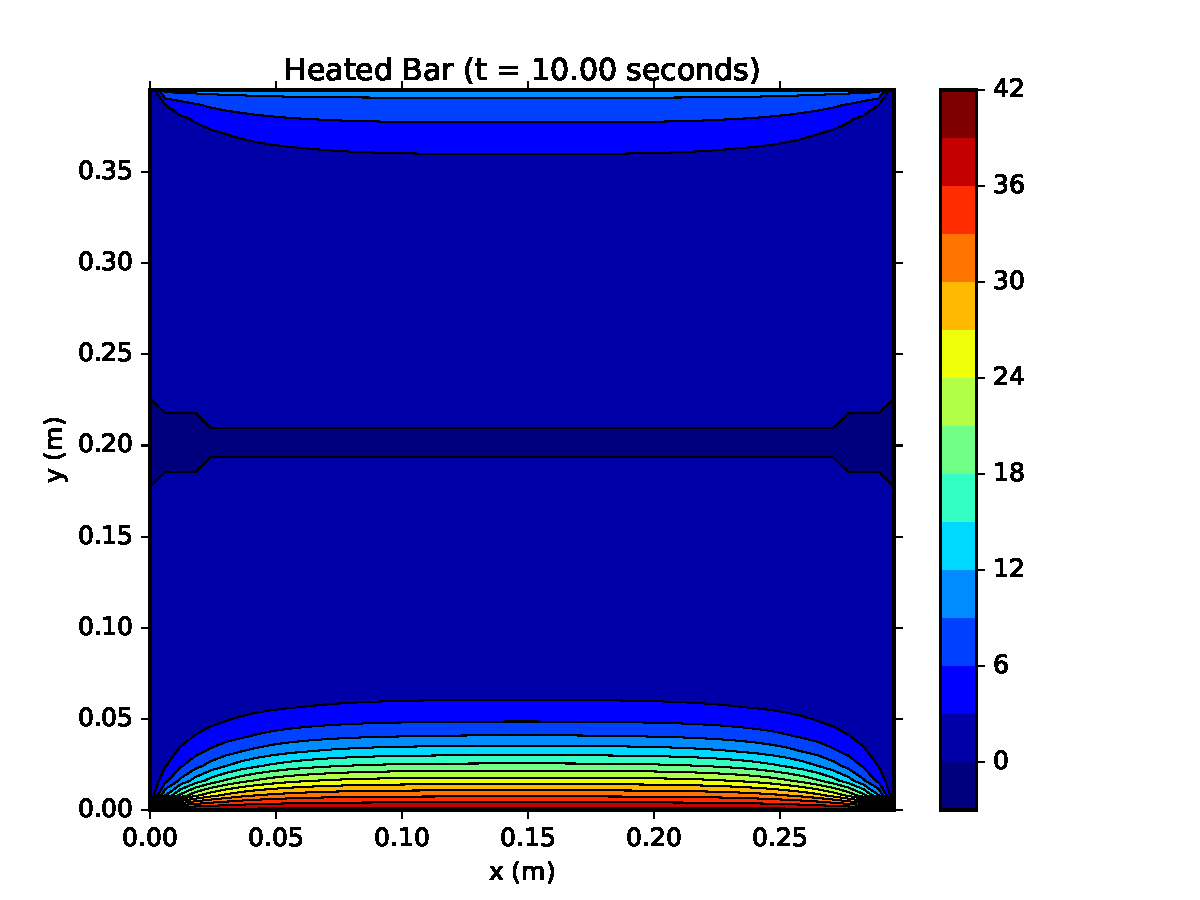
\includegraphics[width=.8\linewidth]{figs/10-00_sec_heat-eq_colorplot.pdf}
\caption{Heated Bar $t=10.00\ s$}
\label{fig:10.0}
\end{figure}

\begin{figure}[H]
\centering
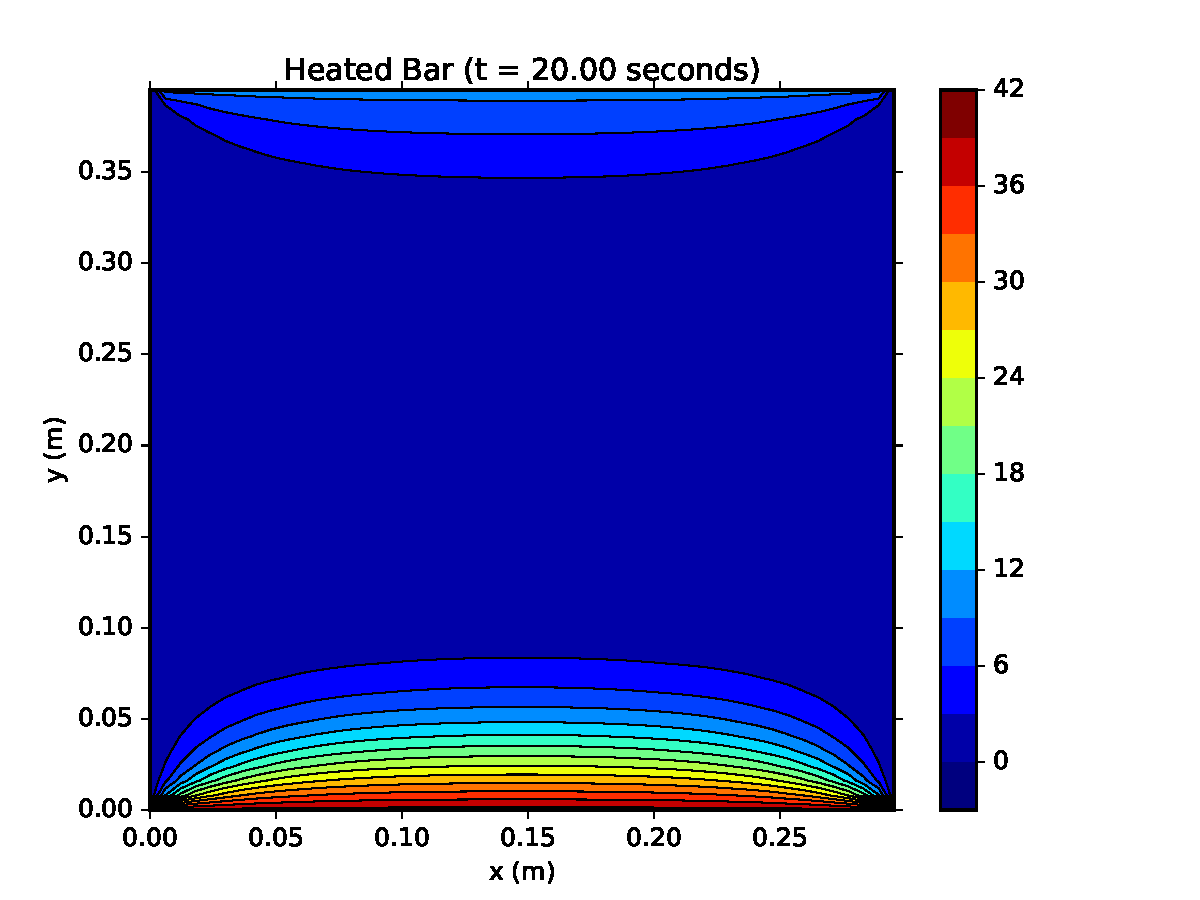
\includegraphics[width=.8\linewidth]{figs/20-00_sec_heat-eq_colorplot.pdf}
\caption{Heated Bar $t=20.00\ s$}
\label{fig:20.0}
\end{figure}

\begin{figure}[H]
\centering
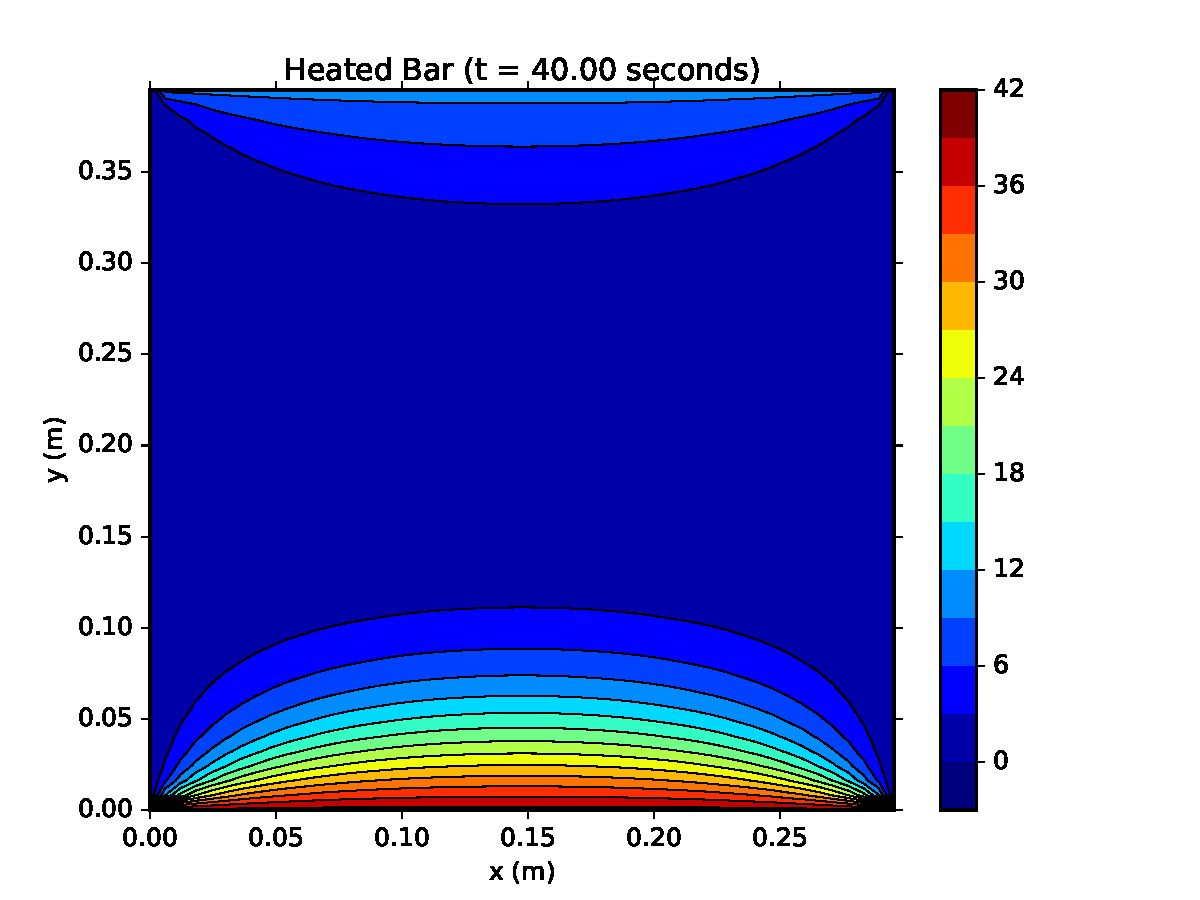
\includegraphics[width=.8\linewidth]{figs/40-00_sec_heat-eq_colorplot.pdf}
\caption{Heated Bar $t=40.00\ s$}
\label{fig:40.0}
\end{figure}

\begin{figure}[H]
\centering
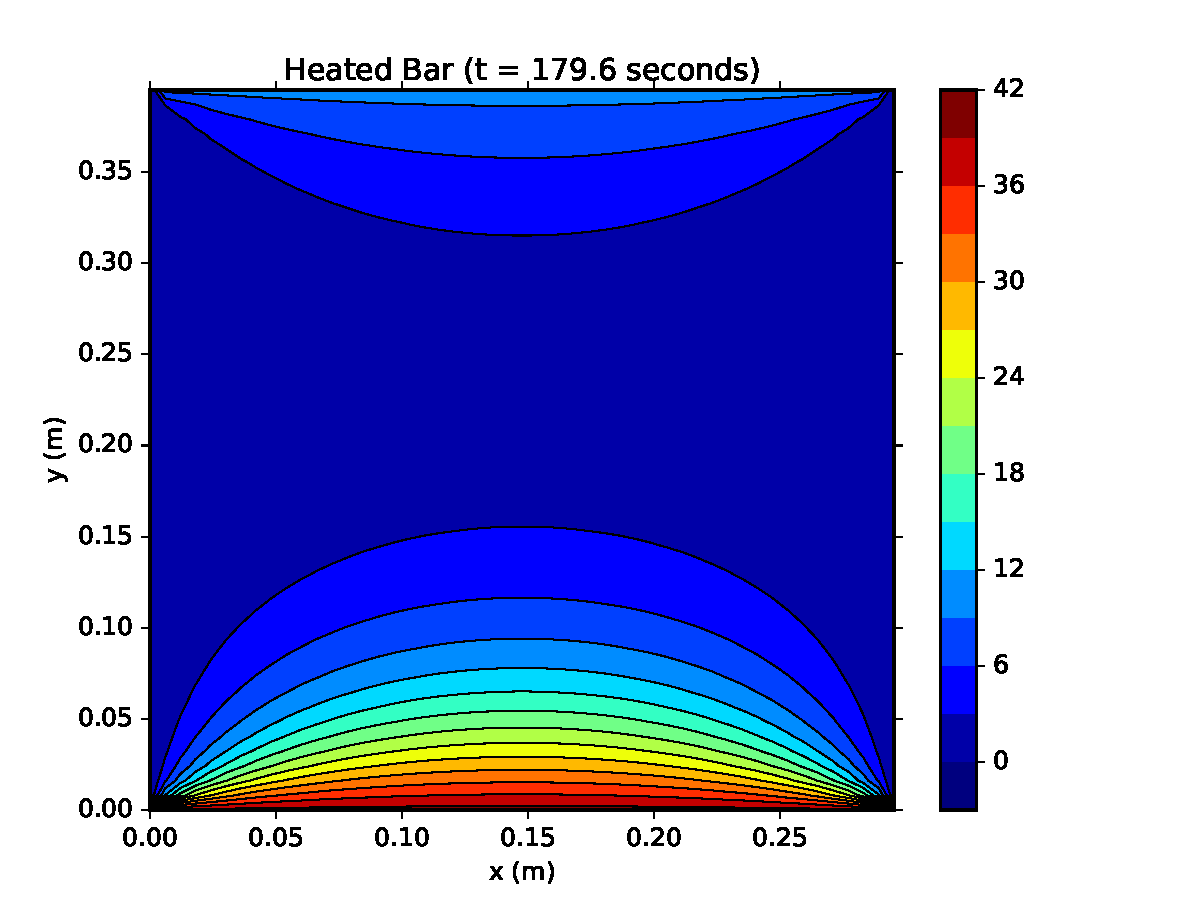
\includegraphics[width=.8\linewidth]{figs/179-6_sec_heat-eq_colorplot.pdf}
\caption{Heated Bar $t=179.6\ s$ (steady state)}
\label{fig:steady_state}
\end{figure}


\end{solution}

\end{questions}

%\begin{thebibliography}{99}
%\end{thebibliography}

\end{document}

%%% Local Variables:
%%% mode: latex
%%% TeX-master: t
%%% End:
